%% main.tex
%% Master document for "Mathemagics: A Field Guide to Random Matrices and Spectral Clustering"
%%
%% Build:
%%   latexmk -pdf  (uses ./latexmkrc which sets shell-escape for minted)
%% Or:
%%   pdflatex --shell-escape main && biber main && pdflatex --shell-escape main && pdflatex --shell-escape main

\documentclass{mathemagics}

% Bibliography (extends the existing refs.bib in Mathematics_Research_Notes)
% \usepackage[style=alphabetic,backend=biber]{biblatex}  % loaded by mathemagics.cls if you uncomment
\addbibresource{refs.bib}

\begin{document}

%%%%%%%%%%%%%%%%%%%%%%%%%%%%%%%%%%%%%%%%%%%%%%%%%%%%%%%%%%%%%%%%%%%%%%%%%%%%%%%
% Frontmatter
%%%%%%%%%%%%%%%%%%%%%%%%%%%%%%%%%%%%%%%%%%%%%%%%%%%%%%%%%%%%%%%%%%%%%%%%%%%%%%%

%% frontmatter/titlepage.tex
%% Half-title + title page

% --- Half-title page (recto, no pagination shown) -----------------------------
\begin{titlepage}
  \centering
  \vspace*{4cm}
  {\LARGE\itshape Mathemagics}\par
  \vspace{14cm}
  \null
\end{titlepage}

% --- Title page ---------------------------------------------------------------
\begin{titlepage}
  \centering
  \vspace*{2.5cm}

  {\fontsize{32}{36}\selectfont\itshape Mathemagics\par}

  \vspace{0.6cm}

  {\Large\scshape A Field Guide to Random Matrices\par}
  \vspace{0.2cm}
  {\Large\scshape and Spectral Clustering\par}

  \vfill

  {\large\rmfamily Arzaan Singh\par}
  \vspace{0.2cm}
  {\itshape under the supervision of\par}
  \vspace{0.2cm}
  {\large\rmfamily Gustavo Didier\par}

  \vspace{1cm}

  {\rmfamily Tulane University\par}

  \vspace{1cm}

  {\rmfamily\itshape Draft \DTMtoday\par}

  \vspace{2cm}
\end{titlepage}

%% frontmatter/colophon.tex
%% Copyright / colophon page

\thispagestyle{empty}
\null\vfill
\noindent
\textit{Mathemagics: A Field Guide to Random Matrices and Spectral Clustering}\par
\vspace{0.5em}
\noindent
\copyright\ \the\year\ Arzaan Singh.\par
\vspace{0.5em}
\noindent
This work is licensed under a Creative Commons Attribution 4.0 International License (CC BY 4.0).\par
\vspace{1em}
\noindent
\textsc{Colophon.} This book was typeset in \LaTeX{} using the \texttt{tufte-book} class as the foundation, with custom theorem environments built on \texttt{tcolorbox} and Python code rendered via \texttt{minted}. The visual identity is inspired by the Tufte school of book design and by Mykel Kochenderfer's and Tim Wheeler's series of textbooks for MIT Press. Source files and Colab notebooks live alongside the book at \texttt{[repo URL placeholder]}.\par
\vspace{1em}
\noindent
First draft: April 2026.\par
\clearpage


\frontmatter

%% frontmatter/preface.tex
%% Preface — explicit four-section structure: who / how / prereqs / outcomes

\chapter*{Preface}
\addcontentsline{toc}{chapter}{Preface}

\PLACEHOLDER{The preface is a tour for the reader, not the author.
A short version follows; the full text will be written once the chapters are filled in.}

\section*{Who this book is for}

This book is written for the curious reader with a basic feel for probability and algebra, who wants to understand why \emph{random matrices} are everywhere in modern data science --- from principal component analysis to deep learning, from finance to wireless communications --- and who has been told the words ``Tracy--Widom,'' ``spiked covariance,'' or ``spectral clustering'' without ever being shown how they fit together.

If you have seen a normal distribution and you know what an eigenvalue is, you have enough background to start. Everything else is built up from scratch.

\section*{How to read this book}

The book supports two reading speeds.

\begin{description}
  \item[The \emph{cliff-notes track}.] Read the chapter opener (\textsc{Where we are} box), the \textsc{Intuition} boxes, the figures, and the \textsc{Chapter recap} at the end. Skip the proofs. You will come away with the conceptual picture in roughly 30\% of the time.
  \item[The \emph{deep-diver track}.] Read everything: definitions, theorems, proofs, examples, simulations, exercises. The book is structured so that every claim is either proved in-line, sketched with a pointer to a full proof in the chapter appendix, or quoted as a standard result with a citation.
\end{description}

The right margin is reserved for asides, small figures, code snippets, and Colab badges. \emph{Asides never carry plot-load} --- if you ignore the entire margin, the proofs still work. Read the margins for context, history, motivation, or the occasional small joke.

\PLACEHOLDER{Cliff-notes track listing: explicit list of which sections to read. To be written once chapters are filled in.}

\section*{What you need to know first}

\begin{itemize}
  \item Some idea of what a random variable is, and what a probability density looks like (we'll re-build all of this from scratch in Part~I, but having seen it once before will speed things up).
  \item Comfort with linear algebra at the level of vectors, matrices, eigenvalues, and a dot product. We re-derive the spectral theorem from scratch in Chapter~6.
  \item Basic Python literacy --- enough to read a NumPy snippet and run a Colab notebook.
\end{itemize}

\section*{What you'll be able to do after}

After reading this book, you will:

\begin{itemize}
  \item Read research papers on random matrix theory and follow the central results without getting stuck on definitions.
  \item Run and interpret simulations of sample covariance matrices, eigenvalue distributions, and Marchenko--Pastur and Tracy--Widom limits.
  \item Recognize the spiked covariance model and the BBP phase transition in real data.
  \item Implement spectral clustering and explain \emph{three} different reasons it works.
\end{itemize}

\section*{A note on style}

The book is written in third person, in the style of polished research notes that have been opened up to a wider audience. Technical content is rigorous; prose is friendly. Cartoon asides exist. The title is a small joke; the math is not.

\bigskip
\noindent\hfill\textit{Arzaan Singh}\par
\noindent\hfill New Orleans, \DTMtoday

%% frontmatter/acknowledgments.tex

\chapter*{Acknowledgments}
\addcontentsline{toc}{chapter}{Acknowledgments}

\PLACEHOLDER{Acknowledgments will be filled in after the first content pass. Names already secured: Gustavo Didier (advisor), Joseph Genzer (whose honors thesis is the structural seed of this book), the Tulane Department of Mathematics.}

%% frontmatter/notation.tex
%% Notation guide. Sortable two-column table.

\chapter*{Notation}
\addcontentsline{toc}{chapter}{Notation}

This is the notation we use throughout the book. The table is sorted roughly by frequency of use.

\PLACEHOLDER{Notation guide will be expanded as chapters are filled in.
The table below is the seed.}

\bigskip
\noindent
\begin{tabular}{@{}ll@{}}
  \toprule
  \textbf{Symbol} & \textbf{Meaning} \\
  \midrule
  $\R, \N, \Z, \Q, \C$ & real, natural, integer, rational, complex numbers \\
  $\E[X]$ & expectation of the random variable $X$ \\
  $\Var(X), \Cov(X, Y)$ & variance, covariance \\
  $\Normal(\mu, \sigma^2)$ & normal (Gaussian) distribution with mean $\mu$, variance $\sigma^2$ \\
  $\Normal_p(\boldsymbol\mu, \Sigma)$ & multivariate normal in $\R^p$ \\
  $\convas, \convp, \convd$ & convergence almost surely / in probability / in distribution \\
  $\Sigma$ & population covariance matrix \\
  $\Shat$ & sample covariance matrix from $n$ observations \\
  $\lambda_i(M)$ & $i$th eigenvalue of the matrix $M$ (ordered) \\
  $\Wishart_p(n, \Sigma)$ & Wishart distribution with $n$ degrees of freedom, scale $\Sigma$ \\
  $W$ & Gaussian Orthogonal Ensemble (GOE) random matrix limit \\
  $f_{\mathrm{MP}}(\lambda)$ & Marchenko--Pastur density \\
  $\mathrm{TW}_1$ & Tracy--Widom law of type 1 ($\beta = 1$) \\
  $\langle u, v \rangle$ & inner product of vectors $u$ and $v$ \\
  $\|M\|_F, \|M\|_{\mathrm{op}}$ & Frobenius and operator norms of a matrix $M$ \\
  $\diag(a_1, \ldots, a_p)$ & diagonal matrix with the listed entries \\
  $I_p$ & $p \times p$ identity matrix \\
  \bottomrule
\end{tabular}

%% frontmatter/dependency-graph.tex
%% Chapter dependency graph — rebuilt to pass the visual audit per STYLE.md §10.1.
%%
%% Layout choice (deliberate): one row per Part, with arrows only WITHIN
%% each row. Reading top-to-bottom implies progression between Parts; the
%% Part labels on the left make this explicit. This eliminates the long
%% cross-row arrows that broke the previous version.

\chapter*{How the chapters depend on each other}
\addcontentsline{toc}{chapter}{Chapter dependency graph}

The chart below is a reading roadmap. Each row is one Part; within each row, an arrow ``\textbf{Ch.\,A} $\to$ \textbf{Ch.\,B}'' means \emph{read Ch.\,A first}. Read top-to-bottom to progress through the book.

If you only have time for the spine, follow the cliff-notes track:
\begin{quote}
  Ch.\,1 $\to$ Ch.\,4 $\to$ Ch.\,7 $\to$ Ch.\,10 $\to$ Ch.\,12 $\to$ Ch.\,17 $\to$ Ch.\,21.
\end{quote}

\bigskip

\begin{fullwidth}
\centering
\begin{tikzpicture}[
  >={Stealth[length=4pt]},
  every node/.style={font=\sffamily},
  chap/.style={
    rectangle, rounded corners=3pt,
    draw=black!60, line width=0.4pt,
    fill=mathemagicsDefBg,
    inner sep=4pt,
    minimum width=2.0cm, minimum height=0.95cm,
    align=center,
    font=\footnotesize\sffamily
  },
  spine/.style={
    rectangle, rounded corners=3pt,
    draw=mathemagicsDef, line width=0.7pt,
    fill=mathemagicsDefBg,
    inner sep=4pt,
    minimum width=2.0cm, minimum height=0.95cm,
    align=center,
    font=\footnotesize\sffamily\bfseries
  },
  needs/.style={->, semithick, draw=black!75, line width=0.5pt,
                shorten >=2pt, shorten <=2pt},
  partlbl/.style={font=\bfseries\small\sffamily, align=right,
                  anchor=east, color=black!65}
]

% ----------------------------------------------------------------
% Row 1: Part I — Foundations of Probability
% ----------------------------------------------------------------
\node[partlbl] at (-0.7, 0)             {Part~I};
\node[spine]   at ( 0.5, 0)        (c1) {Ch.\,1\\RVs};
\node[chap]    at ( 3.0, 0)        (c2) {Ch.\,2\\MGF/CF};
\node[chap]    at ( 5.5, 0)        (c3) {Ch.\,3\\Conv.};
\node[spine]   at ( 8.0, 0)        (c4) {Ch.\,4\\CLT};

\draw[needs] (c1) -- (c2);
\draw[needs] (c2) -- (c3);
\draw[needs] (c3) -- (c4);

% ----------------------------------------------------------------
% Row 2: Part II — From Numbers to Vectors and Matrices
% ----------------------------------------------------------------
\node[partlbl] at (-0.7, -1.6)            {Part~II};
\node[chap]    at ( 0.5, -1.6)      (c5) {Ch.\,5\\Vectors};
\node[chap]    at ( 3.0, -1.6)      (c6) {Ch.\,6\\Linalg};
\node[spine]   at ( 5.5, -1.6)      (c7) {Ch.\,7\\PSD};

\draw[needs] (c5) -- (c6);
\draw[needs] (c6) -- (c7);

% ----------------------------------------------------------------
% Row 3: Part III — Sample Covariance Matrices
% ----------------------------------------------------------------
\node[partlbl] at (-0.7, -3.2)             {Part~III};
\node[chap]    at ( 0.5, -3.2)       (c8) {Ch.\,8\\SCM};
\node[chap]    at ( 3.0, -3.2)       (c9) {Ch.\,9\\Eig.\,conv.};
\node[spine]   at ( 5.5, -3.2)      (c10) {Ch.\,10\\Wishart};

\draw[needs] (c8) -- (c9);
\draw[needs] (c9) -- (c10);

% ----------------------------------------------------------------
% Row 4: Part IV — Eigenvalue Fluctuations in Fixed Dimension
% ----------------------------------------------------------------
\node[partlbl] at (-0.7, -4.8)             {Part~IV};
\node[chap]    at ( 0.5, -4.8)      (c11) {Ch.\,11\\Joint CLT};
\node[spine]   at ( 3.0, -4.8)      (c12) {Ch.\,12\\Two regimes};
\node[chap]    at ( 5.5, -4.8)      (c13) {Ch.\,13\\Eigvecs};
\node[chap]    at ( 8.0, -4.8)      (c14) {Ch.\,14\\GOE};

\draw[needs] (c11) -- (c12);
\draw[needs] (c12) -- (c13);
\draw[needs] (c13) -- (c14);

% ----------------------------------------------------------------
% Row 5: Part V — High-Dimensional Phenomena
% ----------------------------------------------------------------
\node[partlbl] at (-0.7, -6.4)             {Part~V};
\node[chap]    at ( 0.5, -6.4)      (c15) {Ch.\,15\\High-dim};
\node[chap]    at ( 3.0, -6.4)      (c16) {Ch.\,16\\MP};
\node[spine]   at ( 5.5, -6.4)      (c17) {Ch.\,17\\TW};
\node[chap]    at ( 8.0, -6.4)      (c18) {Ch.\,18\\Q-Q};

\draw[needs] (c15) -- (c16);
\draw[needs] (c16) -- (c17);
\draw[needs] (c17) -- (c18);

% ----------------------------------------------------------------
% Row 6: Part VI — Spikes and Spectral Clustering
% ----------------------------------------------------------------
\node[partlbl] at (-0.7, -8.0)             {Part~VI};
\node[chap]    at ( 0.5, -8.0)      (c19) {Ch.\,19\\Spikes};
\node[chap]    at ( 3.0, -8.0)      (c20) {Ch.\,20\\BBP};
\node[spine]   at ( 5.5, -8.0)      (c21) {Ch.\,21\\Spec.\,Clust.};

\draw[needs] (c19) -- (c20);
\draw[needs] (c20) -- (c21);

% ----------------------------------------------------------------
% Legend
% ----------------------------------------------------------------
\node[font=\footnotesize\itshape\sffamily, anchor=west, color=black!65]
  at (-0.7, -9.4)
  {Bordered nodes are on the cliff-notes spine.};

\end{tikzpicture}
\end{fullwidth}

\bigskip

\noindent\textit{The graph is intentionally lossy --- it shows the within-Part reading order, not every cross-reference. When in doubt, the table of contents always works.}


\tableofcontents

%%%%%%%%%%%%%%%%%%%%%%%%%%%%%%%%%%%%%%%%%%%%%%%%%%%%%%%%%%%%%%%%%%%%%%%%%%%%%%%
% Mainmatter
%%%%%%%%%%%%%%%%%%%%%%%%%%%%%%%%%%%%%%%%%%%%%%%%%%%%%%%%%%%%%%%%%%%%%%%%%%%%%%%

\mainmatter

% --- Part 0: Prelude -----------------------------------------------------
%% parts/part0-prelude.tex
\part*{Prelude}
\addcontentsline{toc}{part}{Prelude}

\begin{fullwidth}
\noindent\textit{An appetizer. Where this book is going, in pictures, with almost no equations.}
\end{fullwidth}

%% chapters/00-prelude.tex
\chapter{An Appetizer}
\label{ch:prelude}

\whereWeAre{%
You're starting at the beginning. This chapter is a tour of the destination --- random matrix theory and spectral clustering --- in pictures, with almost no math. After the tour, the rest of the book builds the machinery to make every picture rigorous.%
}

\PLACEHOLDER{The prelude. A short, picture-driven tour of where the book is going. To be written last, after the rest of the book is drafted, so it can promise exactly the punchlines we deliver.}

\section{Random matrices, in two pictures}
\PLACEHOLDER{Marchenko--Pastur picture; spike-detected-by-PCA picture.}

\section{Why the journey starts with coin flips}
\PLACEHOLDER{Argument that even Marchenko--Pastur eventually reduces to a CLT-flavored statement.}

\section{What you'll be able to do at the end}
\PLACEHOLDER{Concrete checklist matching the preface.}

\chapterRecap{%
\begin{itemize}
  \item \PLACEHOLDER{Three bullet teasers.}
\end{itemize}%
}


% --- Part I: Foundations of Probability ----------------------------------
%% parts/part1-foundations.tex
\part{Foundations of Probability}

\begin{fullwidth}
\noindent\textit{We start with the bare minimum. What is a random variable, what is its distribution, how do we summarize it, and what happens when we add many of them up? Part~I builds the probability vocabulary that the rest of the book leans on.}

\medskip
\noindent\textsc{Chapters in this part:} 1.~Random Variables \quad 2.~Generating Functions \quad 3.~Convergence \quad 4.~The Central Limit Theorem.
\end{fullwidth}

%% chapters/01-random-variables.tex
%% Chapter 1: Random Variables, A Working Vocabulary
%%
%% Section status:
%%   §1.0  Chapter opener + whereWeAre   DONE  (audit pass v0.4)
%%   §1.1  Sample spaces, outcomes, X    DONE  (audit pass v0.4 — anchors, cartoons, hints)
%%   §1.2  Distributions: PMF / PDF / CDF  placeholder
%%   §1.3  Expectation and variance        placeholder
%%   §1.4  Independence and joint distributions  placeholder
%%   §1.5  Brief warm-ups + chapter recap  placeholder

\chapter{Random Variables: A Working Vocabulary}
\label{ch:rvs}

\whereWeAre{%
This is the first chapter of the book. Everything that follows, moment generating functions, the central limit theorem, sample covariance matrices, eigenvalue fluctuations, and ultimately spectral clustering, is built on top of the language we develop here.\\[0.3em]
By the end of this chapter the reader will be able to: define random variables and their distributions cleanly, compute expectations and variances of all the running examples (Bernoulli, Binomial, Normal, Exponential), and recognize when two random variables are independent. The chapter assumes only basic high-school algebra and a willingness to draw a few pictures.%
}

% --- Page 11 chapter-opener cartoon -----------------------------------------
% AI-IMAGE SLOT: figures/ch01/wizard-comic.png
% Until that file exists, the TikZ fallback (\wizardHatCartoon) renders.
%
% PROMPT FOR THE IMAGE GENERATOR
% ------------------------------
% A 4-panel hand-drawn comic strip in the style of Calvin and Hobbes (Bill
% Watterson) or Sandra Boynton, soft pastel colors, warm friendly characters.
%
%   Panel 1: A young wizard character with a tall pointed hat (lilac purple,
%            roughly #8273A8) holds up a coin, looking curious. Speech
%            bubble: "Heads or tails?"
%
%   Panel 2: The wizard tosses the coin high in the air. The coin spins
%            mid-air with motion lines. The wizard looks up, expectant.
%
%   Panel 3: The coin lands on a table, balanced perfectly on its edge.
%            The wizard's eyes go wide in surprise.
%
%   Panel 4: The wizard scribbles on a chalkboard the equation
%            "P(edge) ~ 0", with a small sweat drop. Speech bubble:
%            "Probability is rigorous magic."
%
% Style: hand-drawn lines, soft pastel fills, warm off-white background
% (#F8F6F2), charcoal-gray ink lines (#2D2D2D), slight texture.  Use
% lilac, mustard, coral, mint, and soft gold accents.  No text outside
% speech bubbles.  Friendly, gently humorous, NOT slick or stylized like
% anime; closer to a children's book illustration that adults would also
% find charming.
%
% Aspect: ~3:4 portrait or 2x2 grid.  Rendered at margin width (~10pc).
% ----------------------------------------------------------------------
\marginnote{%
\centering
\anchorDot{1}\,\sffamily\footnotesize\scshape Mathemagics\par
\smallskip
\artOrTikz{figures/ch01/wizard-comic.png}{\wizardHatCartoon}\par
\smallskip
\itshape\footnotesize Probability is rigorous magic: we name the unknown, weigh it, and pull conclusions out of it.
}

Probability is the language\anchorDot{1} we use when we want to say something precise about a quantity that is uncertain. The outcome of a coin flip, the height of a randomly chosen person, the largest eigenvalue of a sample covariance matrix; all of these vary across repetitions of the experiment, and probability supplies the vocabulary for describing how. The unit of vocabulary is the \vocab{random variable}: a single number whose value is unknown until the experiment is run. This chapter builds that vocabulary from scratch and trains the running examples that the rest of the book will lean on.

\section{Sample spaces, outcomes, and the function we call \texorpdfstring{$X$}{X}}
\label{sec:rvs-samplespace}

Before we can define a random variable, we need to be precise about what it ``randomizes over.''\anchorDot{2} That requires three pieces:

\begin{enumerate}
\item an \vocab{experiment}, the act whose result is uncertain;
\item the \vocab{sample space} $\Omega$, the set of all possible outcomes of the experiment;
\item a \vocab{probability function} $\Prob$ that assigns a number in $[0,1]$ to events (i.e., subsets of $\Omega$), with $\Prob(\Omega) = 1$.
\end{enumerate}

% --- Page 12 margin: historical aside FIRST, then experiments ---------------
\asideHistorical{\anchorDot{2}\, The modern definition of a random variable as a function on a sample space is due to Andrey Kolmogorov, in his 1933 monograph \emph{Foundations of the Theory of Probability}. Before Kolmogorov, ``random'' was a word in search of a definition.}

\marginGap

\marginnote{%
\centering
\anchorDot{3}\,\sffamily\footnotesize\scshape Three running experiments\par
\medskip
{\renewcommand{\arraystretch}{2.2}%
\begin{tabular}{@{}c@{\quad}l@{}}
\coinbig{H}      & \footnotesize coin: $2$ outcomes\\
\diebig{3}       & \footnotesize die: $6$ outcomes\\
\tapeMeasureIcon & \footnotesize tape measure: a continuum
\end{tabular}}%
}

The simplest example is a single coin flip.\anchorDot{3} The experiment is the flip; the sample space is $\Omega = \{H, T\}$; and the probability function (for a fair coin) is $\Prob(H) = \Prob(T) = \tfrac{1}{2}$. The outcomes here are just the labels $H$ and $T$. They are not numbers, they are labels for possibilities.

Often we care less about the labels themselves than about a number we can compute from them. For two coin flips, we may care about the \emph{number of heads}; for the roll of two dice, we may care about the \emph{sum}; for a clinical trial, we may care about whether a patient recovered or not. In each case there is a function that takes an outcome and returns a number. That function is the random variable.\anchorDot{4}

\begin{definition}{Random variable}{rv}
\anchorDot{1}\,Let $\Omega$ be a sample space. A \emph{random variable} on $\Omega$ is a function $X : \Omega \to \R$ that assigns to each outcome $\omega \in \Omega$ a real number $X(\omega)$.\footnotemark
\end{definition}
\footnotetext{In a fully rigorous treatment we would also require $X$ to be \emph{measurable}; this technical condition becomes relevant only when $\Omega$ is uncountable. Appendix~D sketches the measure-theoretic framework for the curious reader.}

\asideMatters{\anchorDot{1}\, Defining $X$ as a function on $\Omega$, rather than just as ``a random number,'' lets us recover \emph{any} numerical question about the experiment by the same mechanism. The number of heads, the number of tails, whether the first flip matched the second; each is a different function on the same $\Omega$.}

\marginGap

\marginnote{%
\centering
\anchorDot{4}\,\sffamily\footnotesize\scshape A random variable as a machine\par
\smallskip
\begin{tikzpicture}[scale=0.55, every node/.style={font=\sffamily\footnotesize}]
  \node[anchor=east] at (-2.6, 0) {$\omega$};
  \draw[->, line width=0.55pt, mathemagicsThm] (-2.5, 0) -- (-1.05, 0);
  \draw[rounded corners=4pt, draw=mathemagicsThm, fill=mathemagicsIntuBg!70,
        line width=0.7pt]
    (-1, -0.85) rectangle (1, 0.85);
  \node[font=\itshape\bfseries\Large, color=mathemagicsDef] at (0, 0) {$X$};
  \draw[draw=mathemagicsThm, line width=0.4pt] (0, 0.95) circle (0.18);
  \foreach \angle in {0,45,90,135,180,225,270,315} {
    \draw[mathemagicsThm, line width=0.3pt]
      (0, 0.95) ++(\angle:0.18) -- ++(\angle:0.08);
  }
  \draw[->, line width=0.55pt, mathemagicsThm] (1.05, 0) -- (2.5, 0);
  \node[anchor=west] at (2.6, 0) {$X(\omega)$};
\end{tikzpicture}\par
\smallskip
\itshape\footnotesize Outcomes go in; numbers come out. The randomness lives in the input, not in the machine.
}

\begin{intuition}
Think of $X$ as a \emph{measurement device}. The randomness lives in $\Omega$; it is the underlying experiment whose outcome we cannot predict. The random variable $X$ does not introduce any new randomness; it just tells you what number you record once an outcome has been drawn.
\end{intuition}

To see what the definition means in practice, take the simplest non-trivial example.

% --- Page 13 margin: cartoon coin at the start of this subsection -----------
% AI-IMAGE SLOT: figures/ch01/coin-cartoon.png
% Until that file exists, the TikZ fallback (\coinCartoon) renders.
%
% PROMPT FOR THE IMAGE GENERATOR
% ------------------------------
% A hand-drawn cartoon coin character with personality, in the style of a
% Sandra Boynton illustration or a friendly children's book.
%
% The coin is a large round shape (cream / pale-yellow #FBF3D9 fill, with a
% charcoal #2D2D2D outline), shown front-on.  The coin has a face: two big
% round eyes (wide open with curiosity), small expressive eyebrows raised
% in question, and a small smile.  The letter "H" is prominently embossed
% on the coin's face below the eyes.
%
% The coin is mid-thought.  To the right, a small thought bubble (white,
% charcoal outline) trails up from the coin's head with two small puffs
% leading up to a larger speech-bubble shape.  Inside the bubble, in a
% friendly serif font, is the equation: "P(H) = 1/2".
%
% Style: warm hand-drawn ink, soft pastel palette, off-white background
% (#F8F6F2).  Charcoal lines, mustard / cream coin body, no harsh shading.
% Inviting, gently humorous.  The coin is being asked a question and is
% genuinely thinking about it.
%
% Aspect: square (1:1).  Rendered at margin width (~10pc).
% ----------------------------------------------------------------------
\marginnote{%
\centering
\anchorDot{5}\,\sffamily\footnotesize\scshape Heads or tails?\par
\smallskip
\artOrTikz{figures/ch01/coin-cartoon.png}{\coinCartoon}\par
\smallskip
\itshape\footnotesize One coin flip is the simplest non-trivial experiment in all of probability.
}

\begin{example}{Number of heads in two coin flips}{two-coin-flips}
\anchorDot{5}\,Flip a fair coin twice in a row. The sample space contains four outcomes,
\[
\Omega \;=\; \{HH,\; HT,\; TH,\; TT\},
\]
each with probability $\tfrac{1}{4}$. Define the random variable
\[
X(\omega) \;=\; \text{the number of heads in } \omega.
\]
Then $X(HH) = 2$, $X(HT) = 1$, $X(TH) = 1$, and $X(TT) = 0$. So $X$ takes its values in $\{0, 1, 2\} \subset \R$. \cref{fig:rv-mapping} draws the function: outcomes on the left, sorted by their image; the real number line on the right; arrows from each outcome to its target, with $HT$ and $TH$ visibly converging at $1$.
\end{example}

\begin{figure}[h]
\centering
\begin{tikzpicture}[
  >={Stealth[length=4.5pt]},
  every node/.style={font=\sffamily},
  outcome/.style={
    font=\footnotesize\sffamily, color=mathemagicsThm,
    inner sep=2pt
  },
  arr/.style={
    ->, thick, draw=mathemagicsIntu, line width=0.55pt,
    shorten >=2pt, shorten <=2pt
  },
  realline/.style={->, line width=0.6pt, draw=mathemagicsThm}
]
\node[font=\itshape\sffamily, color=mathemagicsThm, anchor=south]
     at (0, 2.25)
     {\large $X = $ ``number of heads in two coin flips''};

\fill[mathemagicsDefBg, rounded corners=8pt]
  (-3.5, -2.0) rectangle (-1.3, 2.0);
\node[font=\sffamily\itshape\bfseries, color=mathemagicsThm,
      anchor=north west]
     at (-3.4, 1.95) {$\Omega$};

\node[outcome] at (-2.4, 1.5)   (hh) {HH};
\node[outcome] at (-2.4, 0.35)  (ht) {HT};
\node[outcome] at (-2.4,-0.35)  (th) {TH};
\node[outcome] at (-2.4,-1.5)   (tt) {TT};

\draw[realline] (3, -1.95) -- (3, 1.95)
  node[above, font=\sffamily, color=mathemagicsThm] {$\R$};
\foreach \y/\lbl in {-1.5/0, 0/1, 1.5/2} {
  \draw[mathemagicsThm, line width=0.5pt] (2.85, \y) -- (3.15, \y);
  \node[right=4pt, font=\footnotesize\sffamily, color=mathemagicsThm]
       at (3.15, \y) {$\lbl$};
}

\draw[arr] (hh.east) -- (2.84, 1.5);
\draw[arr] (ht.east) -- (2.84, 0);
\draw[arr] (th.east) -- (2.84, 0);
\draw[arr] (tt.east) -- (2.84,-1.5);

\node[font=\itshape\sffamily, color=mathemagicsIntu, above=1pt]
     at (0.2, 1.5) {$X$};

\end{tikzpicture}
\caption[The random variable $X$ as a function from $\Omega$ to $\R$.]{The random variable $X$ assigns to every outcome $\omega \in \Omega$ a real number $X(\omega)$. Outcomes that share a value share a target on the line: here $HT$ and $TH$ both map to $1$, which is why $\Prob(X{=}1) = \tfrac{1}{2}$. Layout adapted from~\citep{nrich-rv}.}
\label{fig:rv-mapping}
\end{figure}

Before moving to a richer example, two notational conventions are worth pinning down. They will be used everywhere in this book.

\begin{definition}{Notation: $X$ versus $x$}{notation}
Capital letters ($X$, $Y$, $Z$, \ldots) denote random variables, the \emph{functions} on $\Omega$. Lowercase letters ($x$, $y$, $z$, \ldots) denote particular real numbers, specific values that those random variables \emph{could} take.
\end{definition}

So when we write $\Prob(X = x)$, we are asking: what is the probability that the random variable $X$ takes the value $x$? In the two-coin example above,
\[
\Prob(X = 0) = \tfrac{1}{4}, \qquad
\Prob(X = 1) = \tfrac{1}{2}, \qquad
\Prob(X = 2) = \tfrac{1}{4}.
\]
The probability $\Prob(X = 1) = \tfrac{1}{2}$ comes from the fact that two of the four equally-likely outcomes ($HT$ and $TH$) map to $1$.

A second example, with a richer sample space, exercises the same pattern.

\marginnote{%
\centering
\anchorDot{2}\,\sffamily\footnotesize\scshape One outcome, sum $= 7$\par
\smallskip
\diebig{3}\quad\diebig{4}\par
\smallskip
\itshape\footnotesize One of six pairs that sum to seven; the others are $(\die{1},\die{6})$, $(\die{2},\die{5})$, $(\die{4},\die{3})$, $(\die{5},\die{2})$, $(\die{6},\die{1})$.
}

\begin{example}{Sum of two dice}{two-dice}
Roll two fair six-sided dice.\anchorDot{2} The sample space contains $36$ ordered pairs:
\[
\Omega = \bigl\{(i, j) : i, j \in \{1, 2, 3, 4, 5, 6\}\bigr\},
\]
each with probability $\tfrac{1}{36}$. Let $X(i, j) = i + j$ be the sum. Then $X$ takes values in $\{2, 3, \ldots, 12\}$, and the probability of each value is the number of $(i, j)$ pairs that sum to it, divided by $36$:
\[
\Prob(X = 2) = \tfrac{1}{36}, \quad \Prob(X = 7) = \tfrac{6}{36}, \quad \Prob(X = 12) = \tfrac{1}{36}.
\]
The full distribution of $X$\anchorDot{3} has the familiar triangular shape: rare on the extremes (only one pair sums to $2$), most likely in the middle (six different pairs sum to $7$). \cref{fig:dice-distribution} plots it.
\end{example}

\begin{marginfigure}
\centering
\anchorDot{3}\par\smallskip
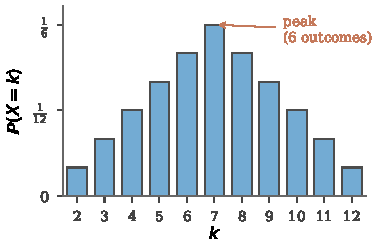
\includegraphics[width=\linewidth]{figures/ch01/dice-distribution.pdf}
\caption{The distribution of $X$ in \cref{ex:two-dice}. The triangular peak at $k = 7$ is no coincidence: of the $36$ equally-likely pairs $(i, j)$, exactly $6$ sum to $7$.}
\label{fig:dice-distribution}
\end{marginfigure}

This is the working pattern. We start from a sample space whose outcomes carry no numerical structure; we define a function $X$ that turns each outcome into a number; and we pull the probabilities forward through $X$ to talk about $\Prob(X = x)$ or, more generally, $\Prob(X \in A)$ for any subset $A$ of $\R$.
\newpage
\subsection*{Brief warm-ups}

\hint{\anchorDot{4}\,How many outcomes do you get from flipping three coins? Try listing them in order, then count those with exactly $k$ heads.}
\begin{warmup}[\coffee{1}]
Three coins are flipped, all fair, all independent.\anchorDot{4} Write down the sample space $\Omega$. Define the random variable $X$ to be the number of heads. List $X(\omega)$ for each $\omega \in \Omega$, and compute $\Prob(X = k)$ for $k = 0, 1, 2, 3$.
\end{warmup}
\begin{warmupSolution}
$\Omega = \{HHH, HHT, HTH, HTT, THH, THT, TTH, TTT\}$, eight outcomes each with probability $\tfrac{1}{8}$. The values of $X$ are $3, 2, 2, 1, 2, 1, 1, 0$ respectively. Counting,
$\Prob(X{=}0) = \tfrac{1}{8}$,
$\Prob(X{=}1) = \tfrac{3}{8}$,
$\Prob(X{=}2) = \tfrac{3}{8}$,
$\Prob(X{=}3) = \tfrac{1}{8}$.
\end{warmupSolution}

\hint{\anchorDot{5}\,A standard deck has $52$ cards, half of them red.}
\begin{warmup}[\coffee{1}]
A single card is drawn from a standard 52-card deck.\anchorDot{5} Define a random variable $Y$ that equals $1$ if the card is red and $0$ if the card is black. What is the sample space, and what is $\Prob(Y = 1)$?
\end{warmup}
\begin{warmupSolution}
$\Omega$ is the set of $52$ cards, each with probability $\tfrac{1}{52}$. The random variable $Y$ takes the value $1$ on the $26$ red cards and $0$ on the $26$ black cards, so $\Prob(Y = 1) = \tfrac{26}{52} = \tfrac{1}{2}$. (This $Y$ is the prototype of the \emph{Bernoulli random variable}, which we will meet again repeatedly starting in \cref{ch:genfunc}.)
\end{warmupSolution}

\hint{\anchorDot{1}\,Out of the $36$ ordered pairs in $\Omega$, how many have $i = j$?}
\begin{warmup}[\coffee{2}]
Re-do \cref{ex:two-dice} but with a different random variable:\anchorDot{1} let $Z(i, j)$ be $1$ if $i = j$ and $0$ otherwise, so $Z$ records whether the two dice show the same face. Compute $\Prob(Z = 1)$.
\end{warmup}
\begin{warmupSolution}
The pairs with $i = j$ are $(1,1), (2,2), (3,3), (4,4), (5,5), (6,6)$, six in total. Each has probability $\tfrac{1}{36}$, so $\Prob(Z = 1) = \tfrac{6}{36} = \tfrac{1}{6}$.
\end{warmupSolution}

\bigskip

% --- §1.1 ENDS HERE ---

% =====================================================================
% §1.2 Distributions: PMFs, PDFs, and CDFs
% =====================================================================

\section{Distributions: PMFs, PDFs, and CDFs}
\label{sec:distributions}

% --- §1.2.1 Bridge + motivation ----------------------------------------------

We have a random variable\anchorDot{1}; how do we summarize its behavior compactly? The full set of probabilities $\Prob(X \in A)$ for every $A \subseteq \R$ is too big to write down directly. We need a single object, a function on $\R$, that contains the same information. There are two natural answers depending on what kind of values $X$ takes.

\marginnote{%
\centering
\anchorDot{1}\,\sffamily\footnotesize\scshape Discrete vs continuous\par
\medskip
\diceVsThermometer\par
\medskip
\itshape\footnotesize Two flavours of randomness, two parallel ways to summarize.
}

A random variable $X$ is \vocab{discrete} if it takes values in a finite or countable set: integers, indicator labels $\{0, 1\}$, the natural numbers. The number of heads in two coin flips and the sum of two dice are both discrete. A random variable $X$ is \vocab{continuous} if its values lie in an interval (or all of $\R$): a length, a temperature, a time. Discrete and continuous random variables share the same definition but require different summaries because of how their probability is allocated. We work through the discrete case first, then the continuous case, then a single unifying object that handles both.

% --- §1.2.2 Discrete: the PMF -------------------------------------------------

\subsection*{Discrete: the probability mass function}

The simplest summary of a discrete random variable lists the probability of every value it can take. That list is the PMF.

\begin{definition}{Probability mass function (PMF)}{pmf}
Let $X$ be a discrete random variable. The \emph{probability mass function} of $X$ is the function $p_X : \R \to [0, 1]$ defined by
\[
p_X(x) \;=\; \Prob(X = x).
\]
A PMF satisfies $p_X(x) \ge 0$ for every $x$, and $\sum_x p_X(x) = 1$, where the sum is over all values $x$ that $X$ can take.
\end{definition}

\begin{intuition}
The PMF places a \emph{weight} at each value the random variable can take, and the weights sum to $1$. Visualised as a bar chart, the height of the bar at $x$ is the probability of seeing exactly that value.
\end{intuition}

\begin{example}{Bernoulli$(p)$}{bernoulli}
A \vocab{Bernoulli random variable} $X \sim \mathrm{Bernoulli}(p)$ takes the value $1$ with probability $p$ and the value $0$ with probability $1 - p$. Its PMF is
\[
p_X(1) = p, \qquad p_X(0) = 1 - p.
\]
The card-colour random variable $Y$ from \cref{ch:rvs} is a Bernoulli with $p = \tfrac{1}{2}$.
\end{example}

\begin{example}{Binomial$(n, p)$}{binomial}
A \vocab{Binomial random variable} $X \sim \mathrm{Bin}(n, p)$ counts the number of successes in $n$ independent Bernoulli$(p)$ trials. Its PMF is
\[
p_X(k) \;=\; \binom{n}{k} p^k (1 - p)^{n - k}, \qquad k = 0, 1, \ldots, n.
\]
The number of heads in $n$ coin flips is exactly $\mathrm{Bin}(n, \tfrac{1}{2})$.
\end{example}

% --- §1.2.3 Continuous: the PDF ----------------------------------------------

\subsection*{Continuous: the probability density function}

The PMF idea breaks down for continuous random variables. Suppose $X$ is the height of a randomly chosen adult, measured in metres. What is $\Prob(X = 1.732)$? The answer is exactly $0$: there are uncountably many possible heights, and no individual real number can carry positive probability without the total exceeding $1$.\anchorDot{2}

\marginnote{%
\centering
\anchorDot{2}\,\sffamily\footnotesize\scshape The density paradox\par
\medskip
\itshape\footnotesize ``What is $\Prob(X = 1.732\,\text{m})$ if $X$ is a height?''\par
\smallskip
$0$.\par
\smallskip
This is not a flaw of the model. There are uncountably many possible heights; no single one can carry positive weight.
}

The fix is to replace point probabilities with a \emph{density}.

\begin{definition}{Probability density function (PDF)}{pdf}
A continuous random variable $X$ has \emph{probability density function} $f_X : \R \to [0, \infty)$ if
\[
\Prob(X \in A) \;=\; \int_A f_X(x)\, dx \qquad \text{for every interval } A \subseteq \R.
\]
A PDF satisfies $f_X(x) \ge 0$ for every $x$ and $\int_{-\infty}^{\infty} f_X(x)\, dx = 1$.
\end{definition}

\begin{intuition}
A PDF is \emph{not} a probability. It is a density, probability per unit of $x$.\anchorDot{3} To turn it into a probability, multiply by $dx$ and integrate over an interval. The total area under the curve is always $1$.
\end{intuition}

\marginnote{%
\centering
\anchorDot{3}\,\sffamily\footnotesize\scshape Density, not probability\par
\smallskip
\itshape\footnotesize $f_X(x)$ can exceed $1$. What must be at most $1$ is the area under the curve over any interval.
}

\begin{example}{Uniform on $[0, 1]$}{uniform}
The \vocab{uniform} random variable $X \sim \mathrm{Uniform}(0, 1)$ has PDF
\[
f_X(x) \;=\; \begin{cases} 1, & 0 \le x \le 1, \\ 0, & \text{otherwise.} \end{cases}
\]
For any subinterval $[a, b] \subseteq [0, 1]$, $\Prob(a \le X \le b) = b - a$.
\end{example}

\begin{example}{Normal $\mathcal{N}(\mu, \sigma^2)$}{normal}
The \vocab{Normal} (or \vocab{Gaussian}) random variable $X \sim \mathcal{N}(\mu, \sigma^2)$ has PDF
\[
f_X(x) \;=\; \frac{1}{\sigma \sqrt{2\pi}} \exp\!\left( -\frac{(x - \mu)^2}{2\sigma^2} \right), \qquad x \in \R.
\]
The bell curve. Its centre is at $\mu$ and its spread is controlled by $\sigma$. Part~I builds toward proving \emph{why} this distribution is so special: it is the universal limit shape of sample averages.
\end{example}

\begin{example}{Exponential$(\lambda)$}{exponential}
An \vocab{Exponential} random variable $X \sim \mathrm{Exp}(\lambda)$ with rate $\lambda > 0$ has PDF
\[
f_X(x) \;=\; \begin{cases} \lambda e^{-\lambda x}, & x \ge 0, \\ 0, & x < 0. \end{cases}
\]
It models waiting times for memoryless events.
\end{example}

\Cref{fig:pdf-curves} plots the three densities side by side at standard parameter values.

\begin{figure}[h]
\centering
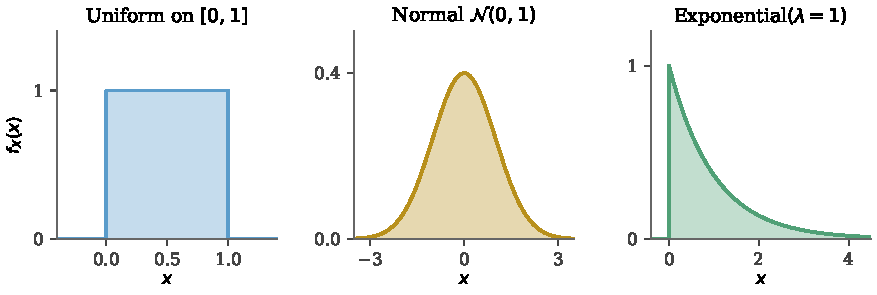
\includegraphics[width=\linewidth]{figures/ch01/pdf-curves.pdf}
\caption[Three PDFs side by side: Uniform, Normal, Exponential.]{Three densities at standard parameter values. The Uniform on $[0,1]$ is constant on its support; the Normal $\mathcal{N}(0,1)$ is the bell curve centred at zero; the Exponential$(1)$ decays from a finite peak at zero. Areas under all three curves are $1$.}
\label{fig:pdf-curves}
\end{figure}

% --- §1.2.4 The CDF: unifying object ----------------------------------------

\subsection*{The cumulative distribution function: a unifying object}

The PMF and PDF are different kinds of objects, applicable to different kinds of random variables. Is there a single function that handles both? Yes. It is the cumulative distribution function.

\begin{definition}{Cumulative distribution function (CDF)}{cdf}
The \emph{cumulative distribution function} of a random variable $X$ is the function $F_X : \R \to [0, 1]$ defined by
\[
F_X(x) \;=\; \Prob(X \le x).
\]
The CDF is non-decreasing, satisfies $\lim_{x \to -\infty} F_X(x) = 0$ and $\lim_{x \to \infty} F_X(x) = 1$, and is right-continuous.
\end{definition}

The CDF is defined for \emph{every} random variable, discrete or continuous. The PMF and PDF are recoverable from it.

\begin{proposition}{Recovering the PMF / PDF from the CDF}{pmf-pdf-from-cdf}
\textit{Let $X$ have CDF $F_X$.}
\begin{itemize}
\item \textit{If $X$ is discrete, the PMF is the jump heights of the CDF: $p_X(x) = F_X(x) - F_X(x^-)$, where $F_X(x^-) = \lim_{y \uparrow x} F_X(y)$.}
\item \textit{If $X$ is continuous and $F_X$ is differentiable at $x$, the PDF is the derivative: $f_X(x) = F_X'(x)$.}
\end{itemize}
\end{proposition}

\begin{proof}[Sketch]
For discrete $X$, the event $\{X \le x\}$ minus the event $\{X < x\}$ is exactly $\{X = x\}$, so the right-side jump of $F_X$ at $x$ has height $\Prob(X = x) = p_X(x)$. For continuous $X$, the fundamental theorem of calculus gives $\frac{d}{dx} \int_{-\infty}^{x} f_X(t)\, dt = f_X(x)$.
\end{proof}

The CDFs of our running examples have three quite different shapes. \Cref{fig:cdf-trio} shows them side by side.

\begin{figure}[h]
\centering
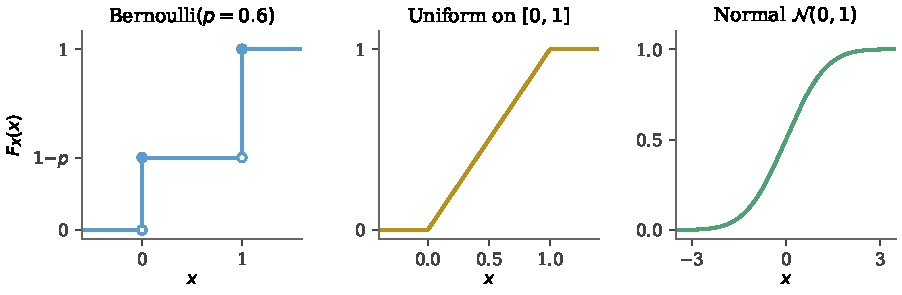
\includegraphics[width=\linewidth]{figures/ch01/cdf-trio.pdf}
\caption[Three CDFs: Bernoulli, Uniform, Normal.]{The CDF of a discrete random variable is a staircase (Bernoulli$(0.6)$, left); the CDF of a uniformly distributed random variable is a linear ramp (Uniform on $[0,1]$, middle); the CDF of a Normal is a smooth S-curve (centre, right). All three are non-decreasing and approach $1$ as $x \to \infty$.}
\label{fig:cdf-trio}
\end{figure}

% --- §1.2.5 Reference table -----------------------------------------------

\subsection*{A reference table of standard distributions}

The book leans on the same handful of standard distributions repeatedly. \Cref{tab:standard-distributions} gathers them in one place; later chapters point back to this table rather than re-defining each distribution.

\begin{table}[h]
\centering
\renewcommand{\arraystretch}{1.4}
\begin{fullwidth}
\footnotesize
\begin{tabular}{@{}llllll@{}}
\toprule
\textbf{Name} & \textbf{Type} & \textbf{Support} & \textbf{PMF / PDF} & \textbf{Mean} & \textbf{Variance} \\
\midrule
Bernoulli$(p)$ & discrete & $\{0, 1\}$ & $p_X(1) = p,\ p_X(0) = 1-p$ & $p$ & $p(1-p)$ \\
Binomial$(n, p)$ & discrete & $\{0, 1, \ldots, n\}$ & $\binom{n}{k} p^k (1-p)^{n-k}$ & $np$ & $np(1-p)$ \\
Geometric$(p)$ & discrete & $\{1, 2, 3, \ldots\}$ & $(1-p)^{k-1} p$ & $1/p$ & $(1-p)/p^2$ \\
Poisson$(\lambda)$ & discrete & $\{0, 1, 2, \ldots\}$ & $e^{-\lambda} \lambda^k / k!$ & $\lambda$ & $\lambda$ \\
\midrule
Uniform$(a, b)$ & continuous & $[a, b]$ & $1/(b-a)$ on $[a, b]$ & $(a+b)/2$ & $(b-a)^2 / 12$ \\
Exponential$(\lambda)$ & continuous & $[0, \infty)$ & $\lambda e^{-\lambda x}$ & $1/\lambda$ & $1/\lambda^2$ \\
Normal$(\mu, \sigma^2)$ & continuous & $\R$ & $\frac{1}{\sigma \sqrt{2\pi}} e^{-(x-\mu)^2 / (2\sigma^2)}$ & $\mu$ & $\sigma^2$ \\
\bottomrule
\end{tabular}
\end{fullwidth}
\caption{The standard distributions used throughout this book. Mean and variance are derived in \cref{ch:genfunc} via moment generating functions.}
\label{tab:standard-distributions}
\end{table}

% --- §1.2.6 Distribution sandbox ------------------------------------------

\subsection*{The distribution sandbox}

Reading a PDF or PMF formula on a page is one thing; watching a simulator throw thousands of samples and seeing the histogram resolve into the theoretical shape is another. \Cref{fig:sandbox-sample} shows a snapshot from the companion Colab notebook: $5{,}000$ samples from $\mathrm{Bin}(20, 0.3)$ on the left and from $\mathcal{N}(0, 1)$ on the right, each plotted against the theoretical PMF or PDF.\anchorDot{4}

\marginnote{%
\centering
\anchorDot{4}\,\sffamily\footnotesize\scshape Distribution sandbox\par
\smallskip
\colablink{Open notebook}{https://github.com/arzaansingh/mathemagics/tree/main/colab-notebooks/ch01-distribution-sandbox.ipynb}\par
\medskip
\itshape\footnotesize Generate samples, compare to theory, vary $N$.
}

\begin{figure}[h]
\centering
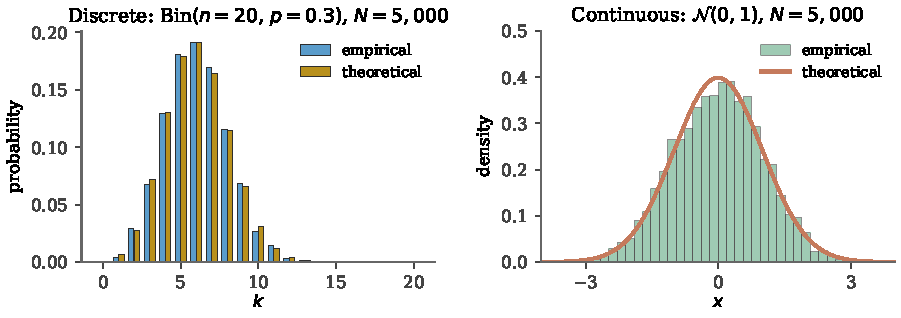
\includegraphics[width=\linewidth]{figures/ch01/sandbox-sample.pdf}
\caption[Sandbox sample: empirical histogram vs theoretical PMF / PDF.]{Empirical histogram (left bars / shaded) overlaid with the theoretical PMF / PDF (right bars / smooth curve) for two distributions, $N = 5{,}000$ samples each. With this many samples the two are visually indistinguishable; with $N = 50$ they would not be.}
\label{fig:sandbox-sample}
\end{figure}

The companion notebook \texttt{ch01-distribution-sandbox.ipynb} runs the same simulation interactively and lets the reader vary $N$, the sample size, to watch the empirical bars converge to the theoretical curves. The convergence is one form of the \emph{law of large numbers}, which we prove in \cref{ch:convergence}.

% --- §1.2.7 Brief warm-ups -----------------------------------------------

\subsection*{Brief warm-ups}

\hint{\anchorDot{5}\,Count the eight equally-likely strings $HHH, HHT, \ldots, TTT$, then group by number of heads.}
\begin{warmup}[\coffee{1}]
Let $X \sim \mathrm{Bin}(3, \tfrac{1}{2})$.\anchorDot{5} List $p_X(k)$ for $k = 0, 1, 2, 3$ and verify they sum to $1$.
\end{warmup}
\begin{warmupSolution}
$p_X(0) = \tfrac{1}{8}$, $p_X(1) = \tfrac{3}{8}$, $p_X(2) = \tfrac{3}{8}$, $p_X(3) = \tfrac{1}{8}$. The four values sum to $1$. (This is also the answer to Warm-up 1 of \cref{sec:rvs-samplespace}, viewed through the PMF.)
\end{warmupSolution}

\hint{\anchorDot{1}\,Integrate the constant density over the interval; equivalently, take the length of the subinterval.}
\begin{warmup}[\coffee{1}]
For $X \sim \mathrm{Uniform}(0, 1)$,\anchorDot{1} compute $\Prob(0.2 \le X \le 0.7)$ and sketch the CDF $F_X$ on the interval $[0, 1]$.
\end{warmup}
\begin{warmupSolution}
$\Prob(0.2 \le X \le 0.7) = 0.5$. The CDF is a linear ramp on $[0, 1]$: $F_X(x) = x$ for $x \in [0, 1]$, with $F_X(x) = 0$ for $x < 0$ and $F_X(x) = 1$ for $x > 1$.
\end{warmupSolution}

\hint{\anchorDot{2}\,A PDF must integrate to $1$ over its full support.}
\begin{warmup}[\coffee{2}]
Suppose $X$ is continuous with PDF $f_X(x) = c x$ for $x \in [0, 2]$, and $f_X(x) = 0$ otherwise.\anchorDot{2} Find the constant $c$.
\end{warmup}
\begin{warmupSolution}
$\int_0^2 c x \, dx = 2c = 1$, so $c = \tfrac{1}{2}$.
\end{warmupSolution}

\hint{\anchorDot{3}\,Integrate $\lambda e^{-\lambda t}$ from $0$ to $x$ to get $F_X(x)$.}
\begin{warmup}[\coffee{2}]
For $X \sim \mathrm{Exp}(\lambda)$,\anchorDot{3} derive the CDF $F_X(x)$ from the PDF $f_X(x) = \lambda e^{-\lambda x}$ on $[0, \infty)$.
\end{warmup}
\begin{warmupSolution}
For $x \ge 0$, $F_X(x) = \int_0^x \lambda e^{-\lambda t} \, dt = 1 - e^{-\lambda x}$. For $x < 0$, $F_X(x) = 0$.
\end{warmupSolution}

\bigskip

% --- §1.2 ENDS HERE; §1.3 onward still placeholder ---

\section{Expectation and variance}
\PLACEHOLDER{§1.3: definition and intuition; linearity of expectation; variance and standard deviation; worked examples on the running distributions.}

\section{Independence and joint distributions}
\PLACEHOLDER{§1.4: two random variables at once; joint and marginal distributions; independence and its consequences; second Colab simulation (joint plots for independent RVs).}

\section{Brief warm-ups and chapter recap}
\PLACEHOLDER{§1.5: 3--5 cross-section warm-ups; chapter recap box.}

\chapterRecap{%
\begin{itemize}
  \item \PLACEHOLDER{Punchline 1.}
  \item \PLACEHOLDER{Punchline 2.}
  \item \PLACEHOLDER{Punchline 3.}
\end{itemize}%
}

\section*{Exercises}
\PLACEHOLDER{8--15 longer exercises; solutions in Appendix A.}

%% chapters/02-generating-functions.tex
\chapter{Generating Functions}
\label{ch:genfunc}

\whereWeAre{%
We've defined random variables and their distributions. Now we ask: what would it look like to package an entire distribution into a single, easy-to-manipulate object? Two such packages turn out to be central in everything that follows: the moment generating function (MGF) and the characteristic function (CF).%
}

\PLACEHOLDER{This chapter has the most mature source material in the existing notes. Pull from \texttt{Mathematics\_Research\_Notes/main.tex}, the MGF and CF sections (lines ~13--585). Use as the canonical reference for visual style of every other chapter.}

\section{Why bundle a distribution into a function?}
\PLACEHOLDER{Motivation: sums of independent RVs become products; moments become derivatives; Laplace/Fourier transform connections.}

\section{The moment generating function}
\PLACEHOLDER{Definition, domain, MGF as a two-sided Laplace transform, MGF generates moments, examples (Bernoulli, Binomial, Poisson, Exponential, Normal).}

\section{Sums of independent random variables}
\PLACEHOLDER{Multiplicativity; Poisson-plus-Poisson example; Normal-plus-Normal example.}

\section{When the MGF fails: characteristic functions}
\PLACEHOLDER{Cauchy distribution as motivation; CF always exists; relationship $\varphi_X(t) = M_X(it)$ when both exist.}

\section{Characteristic function as Fourier transform}
\PLACEHOLDER{Fourier and Fourier--Stieltjes viewpoint.}

\section{Brief warm-ups}
\PLACEHOLDER{3--5 short questions with immediate answers.}

\chapterRecap{%
\begin{itemize}
  \item \PLACEHOLDER{MGFs encode distributions analytically and turn sums into products.}
  \item \PLACEHOLDER{CFs always exist; MGFs sometimes don't.}
  \item \PLACEHOLDER{Both will be the engine of the CLT in Chapter~4.}
\end{itemize}%
}

\section*{Exercises}
\PLACEHOLDER{8--15 longer exercises; solutions in Appendix A.}

%% chapters/03-convergence.tex
\chapter{Convergence: How Sequences of Random Things Settle Down}
\label{ch:convergence}

\whereWeAre{%
A single random variable is one thing; a \emph{sequence} of random variables is the entry point into asymptotic statistics. Three different notions of ``settling down'' coexist, almost surely, in probability, in distribution, with a clean implication chain between them.%
}

\PLACEHOLDER{Sources: existing main.tex `Modes of Convergence' section; Joseph thesis Section 2.2; Casella \& Berger Section 5.5.}

\section{Almost sure convergence}
\PLACEHOLDER{Definition, sample-path interpretation, examples (shifted RVs, $X + 1/n$).}

\section{Convergence in probability}
\PLACEHOLDER{Definition, contrast with a.s.\, the canonical Borel--Cantelli counterexample.}

\section{Markov's and Chebyshev's inequalities}
\PLACEHOLDER{Statements, proofs, used in the WLLN.}

\section{The Weak Law of Large Numbers}
\PLACEHOLDER{Statement, Chebyshev-based proof.}

\section{Convergence in distribution}
\PLACEHOLDER{Definition via CDFs, contrast with the other modes, why it's the right notion for the CLT.}

\section{The implication chain}
\PLACEHOLDER{a.s.\ $\Rightarrow$ in prob $\Rightarrow$ in dist; converses fail.}

\section{Brief warm-ups}
\PLACEHOLDER{3--5 short questions with immediate answers.}

\chapterRecap{%
\begin{itemize}
  \item \PLACEHOLDER{Three modes, ordered from strongest to weakest.}
  \item \PLACEHOLDER{Markov + Chebyshev are the technical workhorses.}
  \item \PLACEHOLDER{Convergence in distribution is what limit theorems are about.}
\end{itemize}%
}

\section*{Exercises}
\PLACEHOLDER{8--15 longer exercises.}

%% chapters/04-clt.tex
\chapter{The Central Limit Theorem}
\label{ch:clt}

\whereWeAre{%
The capstone of Part~I. Lévy's continuity theorem hands us a tool to convert any pointwise statement about characteristic functions into a statement about convergence in distribution. We use it to prove the CLT --- which sits behind essentially every statement in the rest of the book.%
}

\PLACEHOLDER{Sources: existing main.tex `Characteristic Functions and Convergence in Distribution' section; the proof is already written there.}

\section{Lévy's continuity theorem}
\PLACEHOLDER{Statement, intuition, proof sketch (full proof can go to chapter appendix).}

\section{The classical CLT, via characteristic functions}
\PLACEHOLDER{Statement, Taylor expansion of the CF, $\sqrt{n}$ scaling explained, conclusion via Lévy.}

\section{Why $\sqrt{n}$? Where does the $\frac{1}{2}$ come from?}
\PLACEHOLDER{Intuition box; the second moment is the first nonzero term in the CF expansion.}

\section{The CLT in pictures}
\PLACEHOLDER{Histogram of standardized means converging to the bell curve; QQ-plot version; small Colab simulation.}

\section{Brief warm-ups}
\PLACEHOLDER{3--5 short questions.}

\chapterRecap{%
\begin{itemize}
  \item \PLACEHOLDER{The CLT is a statement about $\sqrt{n}$-scaled fluctuations.}
  \item \PLACEHOLDER{Lévy's theorem is the bridge between CFs and distributional convergence.}
  \item \PLACEHOLDER{This Gaussian universality is one of two big universality phenomena in this book; the other --- Tracy--Widom --- waits in Part~V.}
\end{itemize}%
}

\section*{Exercises}
\PLACEHOLDER{8--15 longer exercises.}


% --- Part II: From Numbers to Vectors and Matrices -----------------------
%% parts/part2-vectors-and-matrices.tex
\part{From Numbers to Vectors and Matrices}

\begin{fullwidth}
\noindent\textit{Random matrix theory only makes sense once you stop thinking about a single random number and start thinking about a whole vector --- or even a whole matrix --- of them. Part~II re-tools the foundations to handle vectors and the matrices that summarize their joint behaviour.}

\medskip
\noindent\textsc{Chapters in this part:} 5.~Random Vectors \quad 6.~A Linear Algebra Refresher \quad 7.~Covariance Matrices.
\end{fullwidth}

%% chapters/05-random-vectors.tex
\chapter{Random Vectors and Joint Distributions}
\label{ch:randomvectors}

\whereWeAre{%
Random matrices are made of random numbers, but more directly, of random \emph{vectors} arranged in rows or columns. Before we can study random matrices, we have to understand what it means for an entire vector of random numbers to have a distribution.%
}

\PLACEHOLDER{Sources: existing main.tex `Random Vectors' subsection; Joseph thesis Sections 2.4 (Defs 2.11--2.14, Prop 2.3, Example 2.10).}

\section{What is a random vector?}
\PLACEHOLDER{Definition; joint CDF as a map $\R^p \to [0,1]$; key properties; marginals via limits.}

\section{Independence in higher dimensions}
\PLACEHOLDER{Joint CDF factors; example (independent exponentials); contrast with the maximally dependent case ($X_1 = X_2$ a.s.).}

\section{The multivariate normal distribution}
\PLACEHOLDER{Density formula; bivariate normal worked out; the special Gaussian fact ``zero covariance implies independence,'' valid only in the Gaussian family.}

\section{Brief warm-ups}
\PLACEHOLDER{3--5 short questions.}

\chapterRecap{%
\begin{itemize}
  \item \PLACEHOLDER{A random vector packages multiple random variables with their joint distribution.}
  \item \PLACEHOLDER{Multivariate normality is the workhorse joint distribution and has special independence properties.}
\end{itemize}%
}

\section*{Exercises}
\PLACEHOLDER{8--15 longer exercises.}

%% chapters/06-linalg-refresher.tex
\chapter{A Linear Algebra Refresher}
\label{ch:linalg}

\whereWeAre{%
We need eigenvalues and eigenvectors --- and we need them \emph{understood}, not just defined. This chapter rebuilds the linear algebra of symmetric matrices from scratch: eigenvalues, the spectral theorem, matrix norms, and the equivalence of all norms in finite dimensions.%
}

\PLACEHOLDER{Sources: existing main.tex spectral-theorem subsection; Gilbert Strang \emph{Introduction to Linear Algebra} for accessible-textbook tone.}

\section{Eigenvalues, eigenvectors, the spectral theorem}
\PLACEHOLDER{From scratch: $Av = \lambda v$, geometric meaning, characteristic polynomial; the spectral theorem $A = Q \Lambda Q^T$ for real symmetric $A$.}

\section{Quadratic forms and what eigenvalues control}
\PLACEHOLDER{The diagonal form $x^T A x = \sum \lambda_i y_i^2$; sign of eigenvalues controls definiteness.}

\section{Matrix norms}
\PLACEHOLDER{Frobenius and operator norms; submultiplicativity; equivalence of norms in finite dimensions.}

\section{Continuity of eigenvalues}
\PLACEHOLDER{Determinant is a polynomial in entries; characteristic polynomial coefficients are continuous; roots of polynomials depend continuously on coefficients; therefore eigenvalues depend continuously on matrix entries. This is the analytic engine of Chapter~9.}

\section{Brief warm-ups}
\PLACEHOLDER{3--5 short questions.}

\chapterRecap{%
\begin{itemize}
  \item \PLACEHOLDER{Spectral theorem: real symmetric $\Leftrightarrow$ rotation-scale-rotation.}
  \item \PLACEHOLDER{All norms equivalent in finite dimensions.}
  \item \PLACEHOLDER{Eigenvalues are continuous functions of the matrix.}
\end{itemize}%
}

\section*{Exercises}
\PLACEHOLDER{8--15 longer exercises.}

%% chapters/07-covariance-psd.tex
\chapter{Covariance Matrices and Positive (Semi-)Definiteness}
\label{ch:covariance}

\whereWeAre{%
We package the joint behaviour of a random vector into a single matrix, the \emph{covariance matrix}, and meet the linear-algebraic constraint that all such matrices share: positive semi-definiteness. This is the algebraic gate keeping our matrices inside a well-behaved corner of matrix space.%
}

\PLACEHOLDER{Sources: existing main.tex `Covariance and Covariance Matrices' subsection.}

\section{Covariance and the covariance matrix}
\PLACEHOLDER{Definition; entrywise structure; symmetry; $p=2$ explicit form.}

\section{Why covariance matrices are PSD}
\PLACEHOLDER{Proof via $v^T \Sigma v = \Var(v^T X) \ge 0$.}

\section{When is a covariance matrix PD?}
\PLACEHOLDER{$\Sigma$ fails to be PD iff some nontrivial linear combination collapses to a constant.}

\section{Eigenvalue characterization}
\PLACEHOLDER{$\Sigma$ PSD iff all eigenvalues $\ge 0$; PD iff strictly $> 0$. Connect to Chapter 6.}

\section{Brief warm-ups}
\PLACEHOLDER{3--5 short questions.}

\chapterRecap{%
\begin{itemize}
  \item \PLACEHOLDER{$\Sigma$ encodes the joint covariance structure as a symmetric PSD matrix.}
  \item \PLACEHOLDER{Eigenvalues $\ge 0$ characterize PSD.}
\end{itemize}%
}

\section*{Exercises}
\PLACEHOLDER{8--15 longer exercises.}


% --- Part III: Sample Covariance Matrices --------------------------------
%% parts/part3-sample-covariance.tex
\part{Sample Covariance Matrices}

\begin{fullwidth}
\noindent\textit{In real life, we never know the population covariance, we estimate it from a finite sample. The \emph{sample covariance matrix} is, on the surface, just a calculation; on closer inspection it is a structured random matrix whose entire spectrum carries statistical information. Part~III treats it as such.}

\medskip
\noindent\textsc{Chapters in this part:} 8.~The Sample Covariance Matrix \quad 9.~Eigenvalue Convergence \quad 10.~The Wishart Distribution.
\end{fullwidth}

%% chapters/08-sample-covariance.tex
\chapter{The Sample Covariance Matrix}
\label{ch:scm}

\whereWeAre{%
In real life $\Sigma$ is unknown; we estimate it from data. The estimator is the \emph{sample covariance matrix}, which on the surface is just an arithmetic average of outer products, but on closer inspection is a structured random matrix whose spectrum carries statistical information.%
}

\PLACEHOLDER{Sources: existing main.tex `Sample Covariance Matrix' subsection.}

\section{From population to sample}
\PLACEHOLDER{Sample mean vector; mean-known-zero case ($\Shat = \frac1n X^T X$); mean-unknown case ($\frac{1}{n-1}$ centered).}

\section{Numerical examples}
\PLACEHOLDER{Toy 2D example with three observations; perfect-correlation example; mean-zero example.}

\section{$\Shat$ as a random matrix}
\PLACEHOLDER{Symmetry; PSD; rank under i.i.d.\ Gaussian assumption (full rank when $n \ge p$).}

\section{Brief warm-ups}
\PLACEHOLDER{3--5 short questions.}

\chapterRecap{%
\begin{itemize}
  \item \PLACEHOLDER{$\Shat$ estimates $\Sigma$ from finite data.}
  \item \PLACEHOLDER{$\Shat$ inherits symmetry and PSD from $\Sigma$.}
  \item \PLACEHOLDER{Treating $\Shat$ as a random matrix is the gateway to the rest of this book.}
\end{itemize}%
}

\section*{Exercises}
\PLACEHOLDER{8--15 longer exercises.}

%% chapters/09-eigenvalue-convergence.tex
\chapter{Eigenvalues Are Continuous Functions of the Matrix}
\label{ch:eigconv}

\whereWeAre{%
This is Joseph's Proposition~3.1: when matrices converge, their eigenvalues converge. In the deterministic, almost-sure, and in-probability flavours, the same continuity argument carries the day. This is the spine on which every later eigenvalue convergence claim hangs.%
}

\PLACEHOLDER{Sources: existing main.tex `Continuation: Sample Covariance Matrices, Norms, and Eigenvalue Convergence' section.}

\section{The logical chain}
\PLACEHOLDER{Determinant continuous (polynomial in entries) $\to$ characteristic polynomial coefficients continuous $\to$ roots continuous $\to$ eigenvalues continuous.}

\section{Three convergence flavours}
\PLACEHOLDER{Deterministic, a.s., in probability. Each follows from the deterministic version applied either pointwise on a measure-1 set or via continuity bounds.}

\section{Sanity check: the $2 \times 2$ case}
\PLACEHOLDER{Explicit eigenvalue formula in 2D; entrywise convergence trivially gives eigenvalue convergence.}

\section{Brief warm-ups}
\PLACEHOLDER{3--5 short questions.}

\chapterRecap{%
\begin{itemize}
  \item \PLACEHOLDER{Matrix convergence implies eigenvalue convergence.}
  \item \PLACEHOLDER{The pipeline is: entries $\to$ coefficients $\to$ roots.}
  \item \PLACEHOLDER{This is the analytic engine for the next several chapters.}
\end{itemize}%
}

\section*{Exercises}
\PLACEHOLDER{8--15 longer exercises.}

%% chapters/10-wishart.tex
\chapter{The Wishart Distribution}
\label{ch:wishart}

\whereWeAre{%
When the data is Gaussian, the unscaled sample covariance matrix has a name: the \emph{Wishart distribution}. It is the multivariate generalization of the chi-square law, and it is the cleanest analytic object in this book.%
}

\PLACEHOLDER{Sources: existing main.tex Wishart sections (continuation Apr 16); Joseph thesis Section 3.2 Def 3.3.}

\section{Definition and density}
\PLACEHOLDER{$S = \sum X_i X_i^T$ for Gaussian $X_i$; the Wishart density formula.}

\section{Dimension one collapses to chi-square}
\PLACEHOLDER{Worked specialization. Why this is natural from the construction.}

\section{Dimension two: structure of the Wishart matrix}
\PLACEHOLDER{Diagonal $\chi_n^2$, off-diagonal $\sum x_i y_i$, basic moment computations.}

\section{Brief warm-ups}
\PLACEHOLDER{3--5 short questions.}

\chapterRecap{%
\begin{itemize}
  \item \PLACEHOLDER{Wishart is the multivariate chi-square.}
  \item \PLACEHOLDER{In dimension 1 it \emph{is} chi-square.}
  \item \PLACEHOLDER{In dimension 2 it has clean structure that powers Chapters 11--14.}
\end{itemize}%
}

\section*{Exercises}
\PLACEHOLDER{8--15 longer exercises.}


% --- Part IV: Eigenvalue Fluctuations in Fixed Dimension -----------------
%% parts/part4-fluctuations.tex
\part{Eigenvalue Fluctuations in Fixed Dimension}

\begin{fullwidth}
\noindent\textit{The sample covariance matrix converges to the population covariance matrix. But \emph{how} does it fluctuate around the limit? The answer depends on whether the population eigenvalues are repeated or distinct --- and the two cases lead to fundamentally different limit laws.}

\medskip
\noindent\textsc{Chapters in this part:} 11.~Joint CLT for Entries \quad 12.~Two Fluctuation Regimes \quad 13.~Eigenvector Convergence \quad 14.~The GOE.
\end{fullwidth}

%% chapters/11-joint-clt-entries.tex
\chapter{Joint Asymptotic Distribution of the Matrix Entries}
\label{ch:jointclt}

\whereWeAre{%
We zoom from the matrix to its entries. The three distinct entries of $\sqrt{n}(\Shat - \Sigma)$ in dimension 2 are jointly asymptotically normal, and we'll compute the exact limiting covariance, including using Isserlis's theorem to verify that the off-diagonal asymptotic covariances vanish.%
}

\PLACEHOLDER{Sources: existing main.tex April 16 + April 17 entry-fluctuation sections.}

\section{The three entries and their marginal CLTs}
\PLACEHOLDER{Variances $2$, $2$, $1$ in the $\Sigma = I_2$ case; $2$, $8$, $2$ in the $\Sigma = \diag(1,2)$ case.}

\section{Isserlis's theorem and the diagonal limit}
\PLACEHOLDER{Wick pairings; off-diagonal covariances vanish; limit is diagonal Gaussian.}

\section{Both cases side by side}
\PLACEHOLDER{Case $\Sigma = I_2$ vs $\Sigma = \diag(1,2)$; same engine, different numbers.}

\section{Brief warm-ups}
\PLACEHOLDER{3--5 short questions.}

\chapterRecap{%
\begin{itemize}
  \item \PLACEHOLDER{Joint CLT for the three distinct entries.}
  \item \PLACEHOLDER{Isserlis kills off-diagonal covariances by parity.}
\end{itemize}%
}

\section*{Exercises}
\PLACEHOLDER{8--15 longer exercises.}

%% chapters/12-two-regimes.tex
\chapter{Distinct vs Repeated Eigenvalues: Two Fluctuation Regimes}
\label{ch:tworegimes}

\whereWeAre{%
The first really surprising fact in the book. The same scaling, $\sqrt n$, gives a Gaussian limit when the population eigenvalues are distinct, but a non-Gaussian (GOE-type) limit when they coincide. The reason is that the eigenvalue map is differentiable in one case and only Lipschitz in the other.%
}

\PLACEHOLDER{Sources: existing main.tex `Continuation: Wishart Matrices...' section + April 17 derivative-of-eigenvalue work.}

\section{Case 1: $\Sigma = I_2$ (repeated eigenvalues)}
\PLACEHOLDER{No Taylor expansion needed; eigenvalues of $\Shat$ are eigenvalues of $W_n / \sqrt n$ shifted by 1; limit law is non-Gaussian.}

\section{Case 2: $\Sigma = \diag(1,2)$ (distinct eigenvalues)}
\PLACEHOLDER{First-order perturbation theory; $d\lambda = u^T(dM)u$; delta method; Gaussian limit with variance 8 (top eigenvalue) and 2 (bottom eigenvalue).}

\section{The derivative-of-eigenvalue calculation explicitly}
\PLACEHOLDER{Three partial derivatives: $\partial \lambda_2 / \partial m_{11}, \partial m_{12}, \partial m_{22}$; gradient $(0,0,1)$ at $\Sigma = \diag(1,2)$.}

\section{Why the same $\sqrt{n}$ gives two different laws}
\PLACEHOLDER{The matrix scaling is universal; the eigenvalue map is what differs. Map smooth $\Rightarrow$ delta method; map only Lipschitz $\Rightarrow$ nonlinear limit.}

\section{Brief warm-ups}
\PLACEHOLDER{3--5 short questions.}

\chapterRecap{%
\begin{itemize}
  \item \PLACEHOLDER{Distinct eigenvalues $\to$ Gaussian fluctuations via the delta method.}
  \item \PLACEHOLDER{Repeated eigenvalues $\to$ GOE-like fluctuations.}
  \item \PLACEHOLDER{Same scaling, two universality classes.}
\end{itemize}%
}

\section*{Exercises}
\PLACEHOLDER{8--15 longer exercises.}

%% chapters/13-eigenvectors.tex
\chapter{Eigenvectors: When They Converge and When They Don't}
\label{ch:eigvecs}

\whereWeAre{%
Convergence of eigenvalues does not imply convergence of eigenvectors. When the limiting eigenvalue is simple, the spectral projector is continuous and a sign convention pins down a converging eigenvector. When eigenvalues coincide, the eigenspace is multi-dimensional and the eigenvectors can rotate freely without changing the matrix limit.%
}

\PLACEHOLDER{Sources: April 17 Gustavo notes (rotation counterexample). Existing main.tex April 17 continuation section.}

\section{Spectral projectors and the continuity argument}
\PLACEHOLDER{Riesz contour formula; isolated eigenvalues give continuous projectors; sign convention.}

\section{When eigenvalues coincide}
\PLACEHOLDER{Eigenspace = whole plane; any basis is an eigenbasis; no canonical limit.}

\section{The rotation counterexample}
\PLACEHOLDER{$S_n = O_n \diag(\lambda_1^{(n)}, \lambda_2^{(n)}) O_n^T$ with $\theta_n = n\pi/2$; $S_n \to I_2$ in operator norm but the eigenvectors rotate.}

\section{Brief warm-ups}
\PLACEHOLDER{3--5 short questions.}

\chapterRecap{%
\begin{itemize}
  \item \PLACEHOLDER{Eigenvector convergence requires eigenvalue isolation.}
  \item \PLACEHOLDER{The rotation counterexample makes the failure tangible.}
\end{itemize}%
}

\section*{Exercises}
\PLACEHOLDER{8--15 longer exercises.}

%% chapters/14-goe.tex
\chapter{The Gaussian Orthogonal Ensemble (GOE)}
\label{ch:goe}

\whereWeAre{%
The non-Gaussian limit law from Chapter 12 has a name: the eigenvalue distribution of the \emph{Gaussian Orthogonal Ensemble}. This chapter formalizes the GOE, derives its joint eigenvalue density, and explains the Vandermonde repulsion factor that makes coincident eigenvalues vanishingly unlikely.%
}

\PLACEHOLDER{Sources: existing main.tex GOE section; Joseph thesis Section 3.2.}

\section{Definition of the GOE}
\PLACEHOLDER{$N \times N$ symmetric, diagonal entries $\Normal(0,2)$, off-diagonal $\Normal(0,1)$, all independent up to symmetry. Construction $H = (G+G^T)/\sqrt{2}$ from i.i.d.\ Gaussian $G$.}

\section{Joint eigenvalue density and the Vandermonde}
\PLACEHOLDER{Density formula with $\prod_{i<j} |\lambda_i - \lambda_j|^{\beta=1}$ factor; explicit $2\times 2$ case.}

\section{Eigenvalue repulsion}
\PLACEHOLDER{The Vandermonde forces the density to vanish on the diagonal $\lambda_1 = \lambda_2$; eigenvalues ``avoid'' each other.}

\section{Why GOE specifically appears in our story}
\PLACEHOLDER{$\sqrt{n}(\Shat - I_p)$ converges to a GOE-like matrix in fixed dimension. Closes the loop with Chapter 12.}

\section{Brief warm-ups}
\PLACEHOLDER{3--5 short questions.}

\chapterRecap{%
\begin{itemize}
  \item \PLACEHOLDER{GOE = $\beta = 1$ symmetric Gaussian ensemble.}
  \item \PLACEHOLDER{Vandermonde factor encodes repulsion.}
  \item \PLACEHOLDER{Limit law for $\sqrt n(\Shat - I_p)$ in fixed $p$ is GOE-shaped.}
\end{itemize}%
}

\section*{Exercises}
\PLACEHOLDER{8--15 longer exercises.}


% --- Part V: High-Dimensional Phenomena ----------------------------------
%% parts/part5-high-dim.tex
\part{High-Dimensional Phenomena}

\begin{fullwidth}
\noindent\textit{Once the dimension $p$ grows together with the sample size $n$, the spectral picture changes completely. The empirical eigenvalue distribution stops collapsing to a single point and instead converges to the \emph{Marchenko--Pastur} law. The largest eigenvalue lives at the edge of the bulk, with fluctuations governed by the \emph{Tracy--Widom} law.}

\medskip
\noindent\textsc{Chapters in this part:} 15.~From Fixed-$p$ to High Dimensions \quad 16.~The Marchenko--Pastur Law \quad 17.~Tracy--Widom \quad 18.~Q--Q Plots.
\end{fullwidth}

%% chapters/15-fixed-to-highdim.tex
\chapter{From Fixed-$p$ to High Dimensions}
\label{ch:fixedtohigh}

\whereWeAre{%
Everything in Part~IV assumed $p$ fixed and $n \to \infty$. That regime is fine for classical statistics, but modern data has $p$ comparable to (or much larger than) $n$. The empirical eigenvalue distribution stops collapsing to a point. This chapter is the gateway to the rest of Part~V.%
}

\PLACEHOLDER{New chapter; pulls from April 17 notes and Joseph thesis Section 3.2 (Prop 3.8).}

\section{What changes when $p/n \to c > 0$}
\PLACEHOLDER{The empirical spectral distribution becomes a continuous law, not a delta.}

\section{Three pictures}
\PLACEHOLDER{$p$ fixed: Dirac at 1; $p/n \to c \in (0,1)$: Marchenko--Pastur on $[\lambda_-, \lambda_+]$; $p > n$: rank deficiency, atom at 0.}

\section{The simplest example of rank deficiency: $p=2, n=1$}
\PLACEHOLDER{$\Shat = X_1 X_1^T$ has $\det = 0$; one eigenvalue is exactly zero.}

\section{Brief warm-ups}
\PLACEHOLDER{3--5 short questions.}

\chapterRecap{%
\begin{itemize}
  \item \PLACEHOLDER{High dimensions = $p$ growing with $n$.}
  \item \PLACEHOLDER{ESD has nontrivial support, not just a single point.}
  \item \PLACEHOLDER{When $p > n$, $\Shat$ is rank-deficient.}
\end{itemize}%
}

\section*{Exercises}
\PLACEHOLDER{8--15 longer exercises.}

%% chapters/16-marchenko-pastur.tex
\chapter{The Marchenko--Pastur Law}
\label{ch:mp}

\whereWeAre{%
The Marchenko--Pastur law is the high-dimensional analogue of ``$\Shat \to I_p$.'' Instead of every eigenvalue converging to 1, the empirical eigenvalue distribution converges to a continuous law on $[(1 - \sqrt c)^2, (1 + \sqrt c)^2]$. This is the universal eigenvalue picture for sample covariance matrices in high dimensions.%
}

\PLACEHOLDER{New chapter; pulls from Joseph thesis Section 3.2 (Prop 3.8); reference: Bai \& Silverstein, Vershynin Ch.~7.}

\section{Statement of the Marchenko--Pastur law}
\PLACEHOLDER{Density formula; support $[\lambda_-, \lambda_+] = [(1-\sqrt c)^2, (1+\sqrt c)^2]$; convergence in distribution of the empirical spectral distribution.}

\section{Three perspectives on why it's true}
\PLACEHOLDER{(1) Stieltjes-transform sketch (intuition only); (2) free-probability free convolution; (3) numerical experiment. Pointer to the rigorous proof in chapter appendix.}

\section{What MP looks like as $c$ varies}
\PLACEHOLDER{$c \to 0$: density concentrates near 1 (recovering fixed-$p$); $c = 1$: hits zero on the left edge; $c > 1$: atom at 0, support shifts.}

\section{Simulation: MP as $N$ grows}
\PLACEHOLDER{Colab box: histogram of $\Shat$ eigenvalues for $p=200, 500, 1000$ overlaid with theoretical density.}

\section{Brief warm-ups}
\PLACEHOLDER{3--5 short questions.}

\chapterRecap{%
\begin{itemize}
  \item \PLACEHOLDER{ESD of $\Shat$ converges to Marchenko--Pastur in the high-dim regime.}
  \item \PLACEHOLDER{Support is $[(1-\sqrt c)^2, (1+\sqrt c)^2]$.}
  \item \PLACEHOLDER{Density vanishes like a square root at the edges, the seed of Tracy--Widom.}
\end{itemize}%
}

\section*{Exercises}
\PLACEHOLDER{8--15 longer exercises.}

%% chapters/17-tracy-widom.tex
\chapter{Tracy--Widom: Fluctuations at the Edge}
\label{ch:tw}

\whereWeAre{%
The Marchenko--Pastur law tells us the largest sample eigenvalue stabilizes at $\lambda_+ = (1 + \sqrt c)^2$. But how does it \emph{fluctuate}? The answer is the most famous law in random matrix theory: the Tracy--Widom distribution, which sits at the edge between two regimes and inherits a $p^{-2/3}$ scaling from the square-root vanishing of the MP density.%
}

\PLACEHOLDER{Sources: April 17 Gustavo notes (TW heuristics + $p^{-2/3}$ derivation); Joseph thesis Section 3.2 (Prop 3.9); Quanta Magazine article for context.}

\section{Two heuristics: edge of two regimes, square-root density}
\PLACEHOLDER{(1) TW lives at the boundary between Vandermonde-repelled bulk and empty exterior. (2) MP density $\sim C(\lambda_+ - \lambda)^{1/2}$ near the edge.}

\section{Heuristic derivation of the $p^{-2/3}$ scaling}
\PLACEHOLDER{The "1/p mass in the interval $[\lambda_{\max}, \lambda_+]$" argument, integrated against $C(\lambda_+ - \lambda)^{1/2}$, gives $\lambda_+ - \lambda_{\max} \sim p^{-2/3}$.}

\section{Statement of the Tracy--Widom limit}
\PLACEHOLDER{$p^{2/3}(\lambda_{\max} - \lambda_+) \xrightarrow{d} \mathrm{TW}_1$, with model-dependent prefactor; properties of TW1 (mean, std, skewness).}

\section{Analogy with the CLT}
\PLACEHOLDER{$\sqrt n$-CLT vs $p^{2/3}$-Tracy-Widom: in both cases, the unique scaling that stabilizes the fluctuation.}

\section{Simulation: TW1 from GOE top eigenvalues}
\PLACEHOLDER{Colab box: simulate top eigenvalue of $N \times N$ GOE for growing $N$; histogram converges to TW1 shape (left-skewed).}

\section{Brief warm-ups}
\PLACEHOLDER{3--5 short questions.}

\chapterRecap{%
\begin{itemize}
  \item \PLACEHOLDER{TW1 is the limiting law of $\lambda_{\max}$ at the spectral edge.}
  \item \PLACEHOLDER{$p^{-2/3}$ scaling falls out of the square-root vanishing of MP.}
  \item \PLACEHOLDER{TW1 is to the spectral edge what the Gaussian is to the sample mean.}
\end{itemize}%
}

\section*{Exercises}
\PLACEHOLDER{8--15 longer exercises.}

%% chapters/18-qq-plots.tex
\chapter{Q--Q Plots as Diagnostics}
\label{ch:qq}

\whereWeAre{%
A Q--Q plot is the workhorse visual tool for asking ``does this sample look Gaussian?'' --- and, more interestingly, ``does this sample look \emph{not} Gaussian?'' This chapter builds Q--Q plots from scratch, applies them to the limit laws of Parts~IV and~V, and uses them to see TW1 differ from the Gaussian.%
}

\PLACEHOLDER{Sources: existing main.tex Q--Q plot section; the existing Colab notebook on TW1 vs Gaussian QQ.}

\section{What a Q--Q plot is and isn't}
\PLACEHOLDER{Theoretical quantiles vs sample quantiles; \emph{not} a CDF plot; reading shape (heavy/light tails, scale, skew).}

\section{Three baselines: Gaussian, Cauchy, exponential means}
\PLACEHOLDER{Gaussian sample vs Gaussian quantile (line); Cauchy sample (heavy tails); standardized exponential means (CLT in pictures).}

\section{Q--Q for sample covariance eigenvalues}
\PLACEHOLDER{Distinct vs repeated case revisited; Q--Q plots distinguish the two regimes visually.}

\section{Q--Q for Tracy--Widom vs Gaussian}
\PLACEHOLDER{Standardized TW1 sample vs $\Normal(0,1)$ quantiles; left-tail dip, right-tail flatness; the asymmetry signature.}

\section{Simulation: full Colab notebook}
\PLACEHOLDER{End-to-end Colab box: GOE simulation, normalization, QQ plot, residual plot, scaling sweep with $N$.}

\section{Brief warm-ups}
\PLACEHOLDER{3--5 short questions.}

\chapterRecap{%
\begin{itemize}
  \item \PLACEHOLDER{Q--Q plots are quantile-vs-quantile, not CDF-vs-CDF.}
  \item \PLACEHOLDER{Departures from $y=x$ encode tail behaviour and skewness.}
  \item \PLACEHOLDER{TW1 vs Gaussian QQ shows the universality class boundary.}
\end{itemize}%
}

\section*{Exercises}
\PLACEHOLDER{8--15 longer exercises.}


% --- Part VI: Spikes and Spectral Clustering -----------------------------
%% parts/part6-spikes-clustering.tex
\part{Spikes and Spectral Clustering}

\begin{fullwidth}
\noindent\textit{When the population covariance is the identity plus a low-rank perturbation, a few eigenvalues escape the Marchenko--Pastur bulk --- if and only if the perturbation is strong enough. This is the BBP phase transition, and it is exactly the mechanism behind \emph{spectral clustering}: the destination this entire book has been pointing at.}

\medskip
\noindent\textsc{Chapters in this part:} 19.~Spiked Covariance Models \quad 20.~The BBP Phase Transition \quad 21.~Spectral Clustering: Three Perspectives.
\end{fullwidth}

%% chapters/19-spiked-covariance.tex
\chapter{Spiked Covariance Models}
\label{ch:spiked}

\whereWeAre{%
The Marchenko--Pastur picture describes the eigenvalues of a sample covariance matrix when the population is isotropic ($\Sigma = I_p$). But what if the population has \emph{structure}, a low-rank ``signal'' on top of isotropic noise? That structure either does or does not produce visible eigenvalue spikes above the bulk; this chapter sets up the question and motivates the answer.%
}

\PLACEHOLDER{Mostly new chapter. Reference: Yale Stat 615 Lecture 9, Vershynin Ch.~7--8.}

\section{The spiked model: noise plus low-rank signal}
\PLACEHOLDER{$\Sigma = I_p + \sum_k \theta_k v_k v_k^T$. PCA motivation. Why this is the canonical model in modern data science.}

\section{Examples in the wild}
\PLACEHOLDER{Factor models in finance, latent semantic analysis, gene expression PCA, deep learning Hessian.}

\section{What a spike "looks like" in simulations}
\PLACEHOLDER{Histograms with spike clearly above the MP bulk; scatter of (sample top eigenvalue, true spike strength).}

\section{Brief warm-ups}
\PLACEHOLDER{3--5 short questions.}

\chapterRecap{%
\begin{itemize}
  \item \PLACEHOLDER{Spiked model = isotropic noise + structured low-rank signal.}
  \item \PLACEHOLDER{Spikes show up in the spectrum as outliers above the MP bulk.}
  \item \PLACEHOLDER{Whether they show up depends on signal strength, BBP transition in Chapter 20.}
\end{itemize}%
}

\section*{Exercises}
\PLACEHOLDER{8--15 longer exercises.}

%% chapters/20-bbp-transition.tex
\chapter{The BBP Phase Transition}
\label{ch:bbp}

\whereWeAre{%
The BBP (Baik--Ben Arous--P\'ech\'e) phase transition is the precise mathematical statement of when a spike escapes the Marchenko--Pastur bulk. There is a critical signal strength below which the spike is invisible (eigenvalue stays at the bulk edge) and above which it becomes detectable (eigenvalue moves outside the bulk). This is a phase transition in the literal mathematical sense.%
}

\PLACEHOLDER{Mostly new chapter. Reference: Yale Stat 615 Lecture 9, original BBP paper.}

\section{Sub-critical and super-critical regimes}
\PLACEHOLDER{Critical strength $\theta^* = \sqrt c$. Below: spike eigenvalue stays at $\lambda_+$. Above: spike eigenvalue at $\theta + c\theta/(\theta - 1)$ or similar formula.}

\section{Three pictures of the transition}
\PLACEHOLDER{Sub-critical histogram, super-critical histogram, $\theta$ sweep showing the phase transition.}

\section{Detectability and PCA}
\PLACEHOLDER{Why this matters: PCA is only useful above the BBP threshold. Below threshold, the top sample eigenvector is essentially random.}

\section{Simulation: BBP transition sweep}
\PLACEHOLDER{Colab box: parameter sweep over $\theta$ with histogram of top sample eigenvalue.}

\section{Brief warm-ups}
\PLACEHOLDER{3--5 short questions.}

\chapterRecap{%
\begin{itemize}
  \item \PLACEHOLDER{BBP gives a sharp threshold for spike detection.}
  \item \PLACEHOLDER{Below threshold: spike invisible.}
  \item \PLACEHOLDER{Above threshold: spike detectable, eigenvalue moves outside the bulk.}
\end{itemize}%
}

\section*{Exercises}
\PLACEHOLDER{8--15 longer exercises.}

%% chapters/21-spectral-clustering.tex
\chapter{Spectral Clustering: Three Perspectives}
\label{ch:specclust}

\whereWeAre{%
The destination. \emph{Spectral clustering} is what happens when you take the spiked-covariance picture seriously: the signal eigenvectors of a similarity matrix, graph Laplacian, or kernel reveal cluster structure in the data. We follow von Luxburg and present the algorithm three different ways, so that if one explanation doesn't click, the other two will.%
}

\PLACEHOLDER{New chapter. Primary source: von Luxburg's \emph{A Tutorial on Spectral Clustering} (the canonical pedagogical reference).}

\section{The algorithm in one paragraph}
\PLACEHOLDER{Build similarity graph; compute graph Laplacian; take its smallest $k$ eigenvectors; cluster the $n$ embedded points with $k$-means.}

\section{Perspective 1: graph cut}
\PLACEHOLDER{Normalized cut interpretation; spectral relaxation of an NP-hard problem.}

\section{Perspective 2: random walk}
\PLACEHOLDER{Random walk on the similarity graph; the Laplacian eigenvectors are stationary modes.}

\section{Perspective 3: perturbation theory}
\PLACEHOLDER{The Laplacian of a block-structured graph has a specific spectrum; perturbations don't break the picture too much. This is where the BBP intuition feeds in directly.}

\section{Why this is the destination of the entire book}
\PLACEHOLDER{The full chain: Gaussian foundations $\to$ random matrices $\to$ spiked covariance $\to$ BBP detectability $\to$ clusters revealed by top eigenvectors. Spectral clustering is exactly the algorithmic payoff.}

\section{Simulation: spectral clustering on a synthetic dataset}
\PLACEHOLDER{Colab box: two-blob dataset, build kernel, compute Laplacian eigenvectors, $k$-means in spectral coordinates.}

\section{Brief warm-ups}
\PLACEHOLDER{3--5 short questions.}

\chapterRecap{%
\begin{itemize}
  \item \PLACEHOLDER{Spectral clustering = top/bottom Laplacian eigenvectors + $k$-means.}
  \item \PLACEHOLDER{Three independent reasons it works.}
  \item \PLACEHOLDER{Random matrix theory is the explanation for \emph{when} it works.}
\end{itemize}%
}

\section*{Exercises}
\PLACEHOLDER{8--15 longer exercises.}


% --- Coda ----------------------------------------------------------------
%% coda/where-to-next.tex

\chapter*{Coda: Where to Next}
\addcontentsline{toc}{chapter}{Coda: Where to Next}

\PLACEHOLDER{This closing chapter is a short tour of the territory beyond
this book. To be filled in after the main chapters are drafted.}

\section*{Universality classes beyond Tracy--Widom}

\PLACEHOLDER{TW is one universality class. There are others (Pearcey, Airy,
sine, $\beta$-ensembles). Brief tour.}

\section*{Multiscale phenomena}

\PLACEHOLDER{Joseph Genzer's honors thesis introduced fractional Brownian
motion and a phase transition at $H = 0.75$. Brief teaser of that storyline.}

\section*{Where this stuff actually shows up}

\PLACEHOLDER{Connections to deep learning (training dynamics, NTK, Hessian
spectra), finance (portfolio risk, factor models), wireless communications
(MIMO capacity), and biology (PCA in genomics).}

\section*{Where to read next}

\PLACEHOLDER{Annotated reading list:
Tao's \emph{Topics in Random Matrix Theory},
Vershynin's \emph{High-Dimensional Probability},
Bai and Silverstein,
Anderson--Guionnet--Zeitouni,
Couillet and Debbah,
the Wikipedia Tracy--Widom article (yes, really),
Joseph's thesis itself.}


%%%%%%%%%%%%%%%%%%%%%%%%%%%%%%%%%%%%%%%%%%%%%%%%%%%%%%%%%%%%%%%%%%%%%%%%%%%%%%%
% Backmatter
%%%%%%%%%%%%%%%%%%%%%%%%%%%%%%%%%%%%%%%%%%%%%%%%%%%%%%%%%%%%%%%%%%%%%%%%%%%%%%%

\backmatter

\appendix

%% appendices/A-solutions.tex
\chapter{Solutions to End-of-Chapter Exercises}
\label{app:solutions}

\PLACEHOLDER{This appendix collects the full solutions to the end-of-chapter exercises. Section per chapter; entry per exercise. Filled in incrementally as chapters are written.}

\section*{Solutions for Chapter 1}
\PLACEHOLDER{To be filled in.}

\section*{Solutions for Chapter 2}
\PLACEHOLDER{To be filled in.}

\section*{Solutions for Chapter 3}
\PLACEHOLDER{To be filled in.}

% ... and so on for chapters 4--21

%% appendices/B-notation.tex
\chapter{Notation Index}
\label{app:notation}

\PLACEHOLDER{The full notation index is here. The frontmatter notation guide is the seed; this appendix is the comprehensive list, sortable by symbol with chapter-of-introduction.}

\bigskip
\noindent
\begin{tabular}{@{}lll@{}}
  \toprule
  \textbf{Symbol} & \textbf{Meaning} & \textbf{First used} \\
  \midrule
  $\R, \N, \Z$ & real, natural, integer numbers & Ch.\ 1 \\
  $\E[X]$ & expectation of $X$ & Ch.\ 1 \\
  $\Var(X)$ & variance of $X$ & Ch.\ 1 \\
  $M_X(t)$ & moment generating function of $X$ & Ch.\ 2 \\
  $\varphi_X(t)$ & characteristic function of $X$ & Ch.\ 2 \\
  $\convas, \convp, \convd$ & convergence (a.s., probability, distribution) & Ch.\ 3 \\
  $\Sigma$ & population covariance matrix & Ch.\ 7 \\
  $\Shat$ & sample covariance matrix & Ch.\ 8 \\
  $\lambda_i(M)$ & $i$th eigenvalue of $M$ & Ch.\ 6 \\
  $\Wishart_p(n, \Sigma)$ & Wishart distribution & Ch.\ 10 \\
  $f_{\mathrm{MP}}$ & Marchenko--Pastur density & Ch.\ 16 \\
  $\mathrm{TW}_1$ & Tracy--Widom type 1 & Ch.\ 17 \\
  \bottomrule
\end{tabular}

\PLACEHOLDER{Expand as chapters are filled in.}

%% appendices/C-code-listings.tex
\chapter{Code Listings and Colab Notebook Index}
\label{app:code}

\PLACEHOLDER{This appendix is a directory of every simulation in the book, with: short description, chapter where it appears, link to the live Colab notebook, and (where short enough) the inline Python code. The point is that a reader can fork a notebook for any experiment in the book in one click.}

\bigskip
\noindent
\begin{tabular}{@{}llll@{}}
  \toprule
  \textbf{Simulation} & \textbf{Chapter} & \textbf{Topic} & \textbf{Notebook} \\
  \midrule
  Sim.\ 4.1 & 4 & CLT in pictures & \PLACEHOLDER{link} \\
  Sim.\ 16.1 & 16 & MP as $N$ grows & \PLACEHOLDER{link} \\
  Sim.\ 17.1 & 17 & TW1 from GOE top eigenvalue & \PLACEHOLDER{link} \\
  Sim.\ 18.1 & 18 & QQ-plot diagnostic suite & \PLACEHOLDER{link} \\
  Sim.\ 20.1 & 20 & BBP transition sweep & \PLACEHOLDER{link} \\
  Sim.\ 21.1 & 21 & Spectral clustering on a synthetic dataset & \PLACEHOLDER{link} \\
  \bottomrule
\end{tabular}

\PLACEHOLDER{Expand as Colab notebooks are written. Each Colab box in the body text should have a matching entry here.}

%% appendices/D-prerequisites.tex
\chapter{Mathematical Prerequisites}
\label{app:prereqs}

\PLACEHOLDER{This appendix collects the bare-minimum prerequisites that the body of the book either assumes or alludes to without developing in full. The level of detail is calibrated as Chapter 1 lands. Topics:}

\begin{itemize}
  \item Sigma-algebras and measurability (sketched at the level needed)
  \item Limits, continuity, $\varepsilon$-$\delta$
  \item Riemann vs Lebesgue integration (one paragraph)
  \item Real analysis essentials (Weierstrass, Bolzano--Weierstrass)
  \item Orthogonal matrices and the orthogonal group $O(n)$
  \item A note on conventions (we use $X^T$ for transpose, etc.)
\end{itemize}

\PLACEHOLDER{Each of these gets one short section. Pointers to the literature (Tao's analysis books, Folland) are given at the end of each section.}

%% appendices/E-bibliography-notes.tex
\chapter{Annotated Reading List}
\label{app:reading}

\PLACEHOLDER{This is not the bibliography (the actual bibliography is at the end of the book in BibTeX). This is the \emph{annotated} reading list: 1--3 sentences per source explaining what it does well and what to read it for. Pattern borrowed from Larry Wasserman's `Bibliographic Remarks' sections in \emph{All of Statistics}.}

\section*{Probability foundations}
\PLACEHOLDER{Casella \& Berger, Feller, Billingsley.}

\section*{Linear algebra}
\PLACEHOLDER{Strang, Horn \& Johnson.}

\section*{Random matrix theory}
\PLACEHOLDER{Tao's \emph{Topics in Random Matrix Theory} (free PDF), Anderson--Guionnet--Zeitouni, Bai \& Silverstein, Couillet \& Debbah.}

\section*{High-dimensional probability}
\PLACEHOLDER{Vershynin \emph{HDP}, Wainwright \emph{HDS}.}

\section*{Spectral clustering}
\PLACEHOLDER{Von Luxburg's tutorial, Ng--Jordan--Weiss, Shi--Malik.}

\section*{Tracy--Widom and the spectral edge}
\PLACEHOLDER{Original Tracy--Widom papers, Edelman \& Sutton expository pieces, the Quanta Magazine article.}

\section*{Applications}
\PLACEHOLDER{Connections to deep learning, finance, biology, short pointers.}

\section*{Joseph Genzer's honors thesis}
\PLACEHOLDER{The structural seed of this book; covers the multiscale phase transition Mathemagics defers to Volume II.}


% Bibliography (auto-generated from refs.bib)
\printbibliography[heading=bibintoc]

% Subject index
%% appendices/F-index.tex
%% Subject index. The actual index entries are scattered throughout the text
%% via \index{...} or \vocab{...} (defined in style/macros.tex).
%% This file just calls \printindex; LaTeX/imakeidx do the rest.

\printindex


\end{document}
